\section{Windows Server 2012}
\subsection{Ajout de fonctionnalités de Windows Server}

Démarrer la machine virtuelle Windows Server 2012. Ouvrir le gestionnaire de serveur (s'ouvre normalement automatiquement lors du démarrage de la machine). Cliquer sur "\textit{Ajouter des rôles et des fonctionnalités}" :
\begin{figure}[h!]
    \begin{center}
        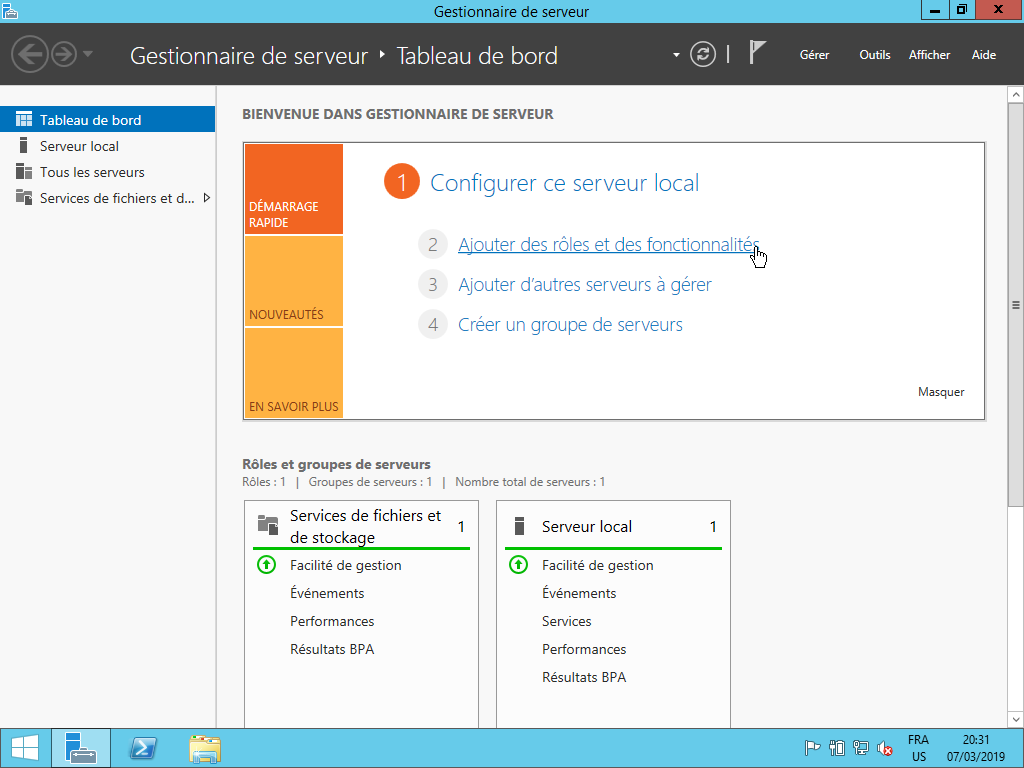
\includegraphics[scale=0.6]{WS2012_Screenshots/17.png}
        \caption{Ajout des rôles et des fonctionnalités sur Windows Server 2012}
        \label{WS2012_Screenshots/17}
    \end{center}
\end{figure}
\FloatBarrier

\newpage
Aller dans la section \textbf{Avant de commencer}, puis cliquer sur \textit{Suivant} :
\begin{figure}[h!]
    \begin{center}
        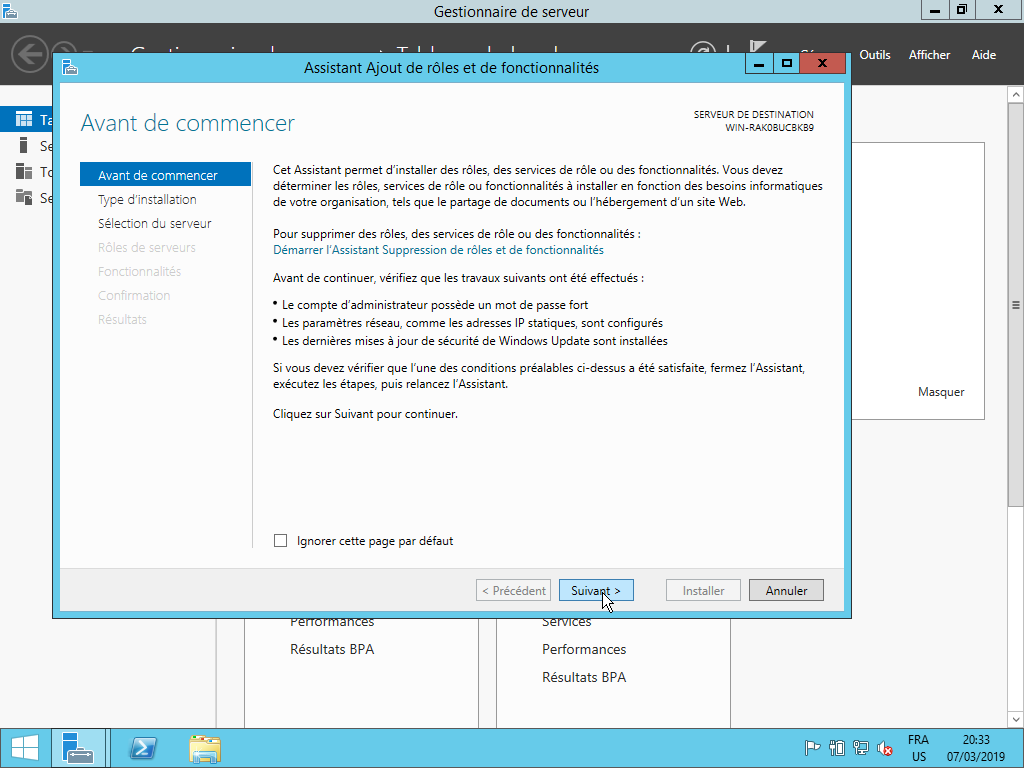
\includegraphics[scale=0.6]{WS2012_Screenshots/18.png}
        \caption{Avant de commencer - Assistant d'ajout de rôles et de fonctionnalités de Windows Server 2012}
        \label{WS2012_Screenshots/18}
    \end{center}
\end{figure}
\FloatBarrier

\newpage
Aller dans la section \textbf{Type d'installation}, sélectionner la première option "\textit{Installation basée sur un rôle ou une fonctionnalité}", puis cliquer sur \textit{Suivant} :
\begin{figure}[h!]
    \begin{center}
        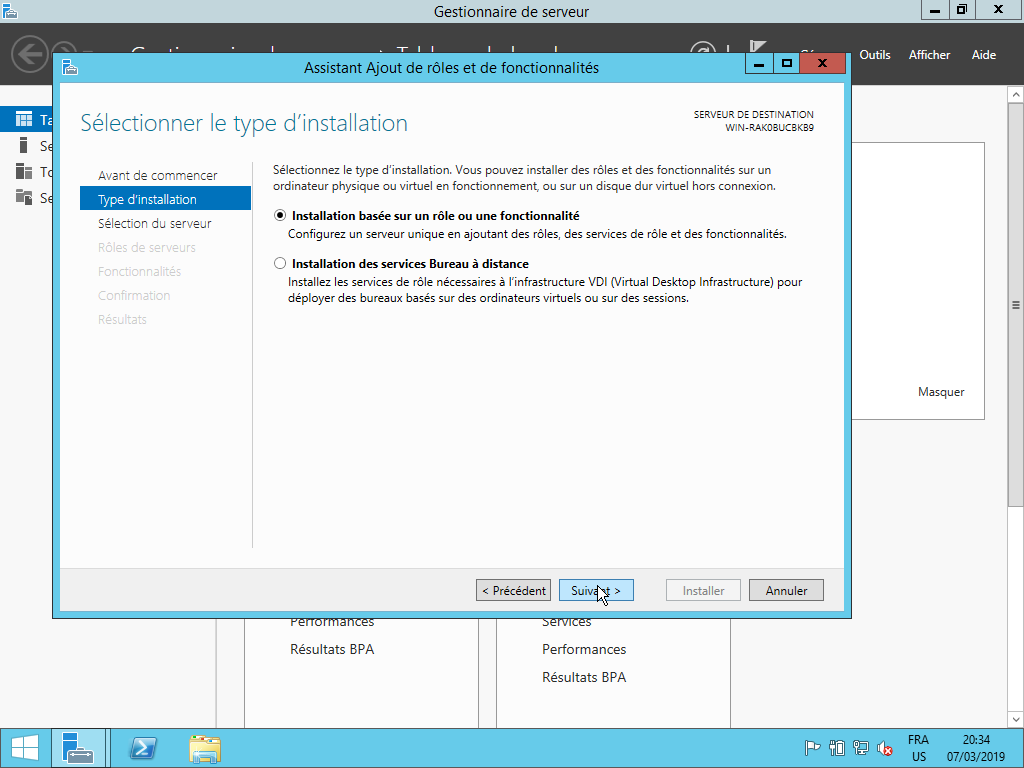
\includegraphics[scale=0.6]{WS2012_Screenshots/19.png}
        \caption{Type d'installation - Assistant d'ajout de rôles et de fonctionnalités de Windows Server 2012}
        \label{WS2012_Screenshots/19}
    \end{center}
\end{figure}
\FloatBarrier

\newpage
Aller dans la section \textbf{Sélection du serveur}. Cocher l'option "Sélectionner un serveur de pool de serveurs". Choisir \textit{DC01.EPITAF.local}, puis cliquer sur \textit{Suivant} :
\begin{figure}[h!]
    \begin{center}
        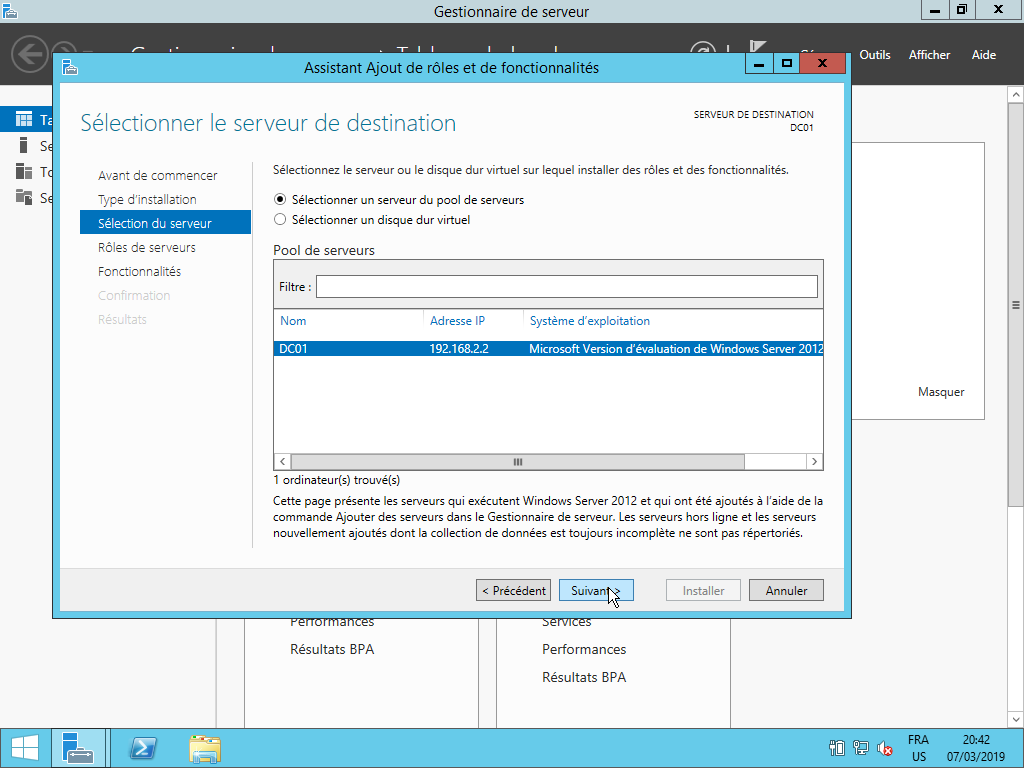
\includegraphics[scale=0.6]{WS2012_Screenshots/20.png}
        \caption{Sélection du serveur - Assistant d'ajout de rôles et de fonctionnalités de Windows Server 2012}
        \label{WS2012_Screenshots/20}
    \end{center}
\end{figure}
\FloatBarrier

\newpage
Aller dans la section \textbf{Rôles de serveurs}. Cocher les options :
\begin{itemize}
    \item Serveur DHCP (installé);
    \item Serveur DNS (installé);
    \item Services AD DS (Installé).
\end{itemize}
Cliquer sur \textit{Suivant}, puis cliquer sur \textit{Ajouter des fonctionnalités} :
\begin{figure}[h!]
    \begin{center}
        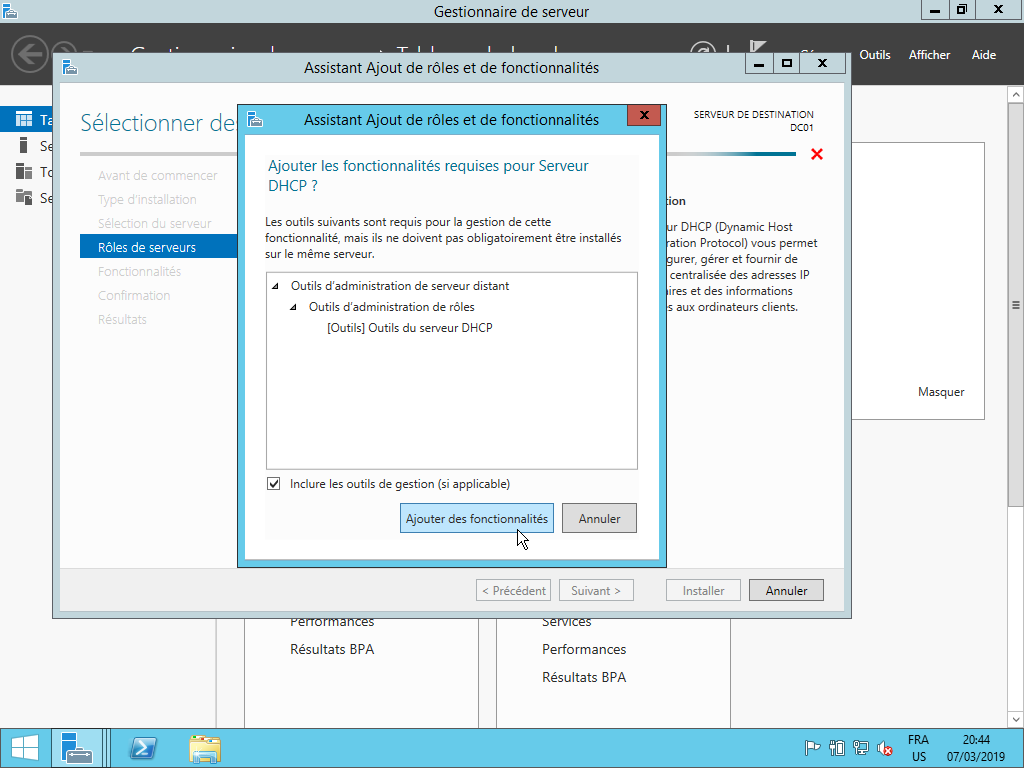
\includegraphics[scale=0.6]{WS2012_Screenshots/21.png}
        \caption{Ajout de DHCP - Assistant d'ajout de rôles et de fonctionnalités de Windows Server 2012}
        \label{WS2012_Screenshots/21}
    \end{center}
\end{figure}
\FloatBarrier

\newpage
Cliquer sur \textit{Ajouter des fonctionnalités} :
\begin{figure}[h!]
    \begin{center}
        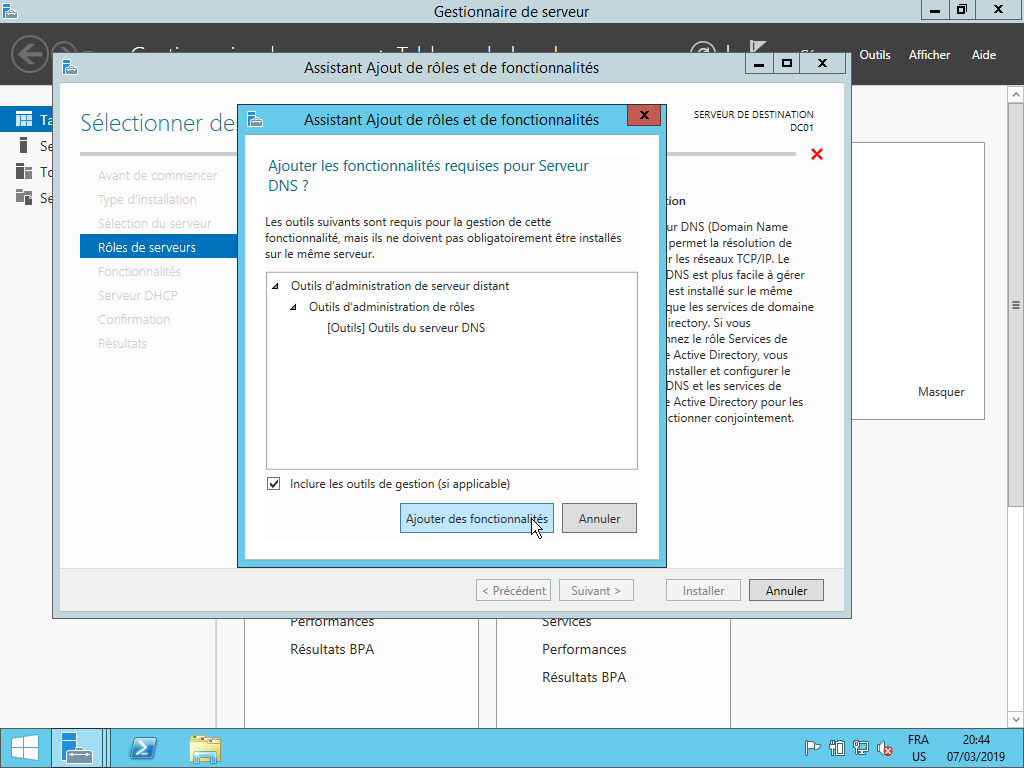
\includegraphics[scale=0.6]{WS2012_Screenshots/22.png}
        \caption{Ajout de DNS - Assistant d'ajout de rôles et de fonctionnalités de Windows Server 2012}
        \label{WS2012_Screenshots/22}
    \end{center}
\end{figure}
\FloatBarrier

\newpage
Cliquer sur \textit{Ajouter des fonctionnalités} :
\begin{figure}[h!]
    \begin{center}
        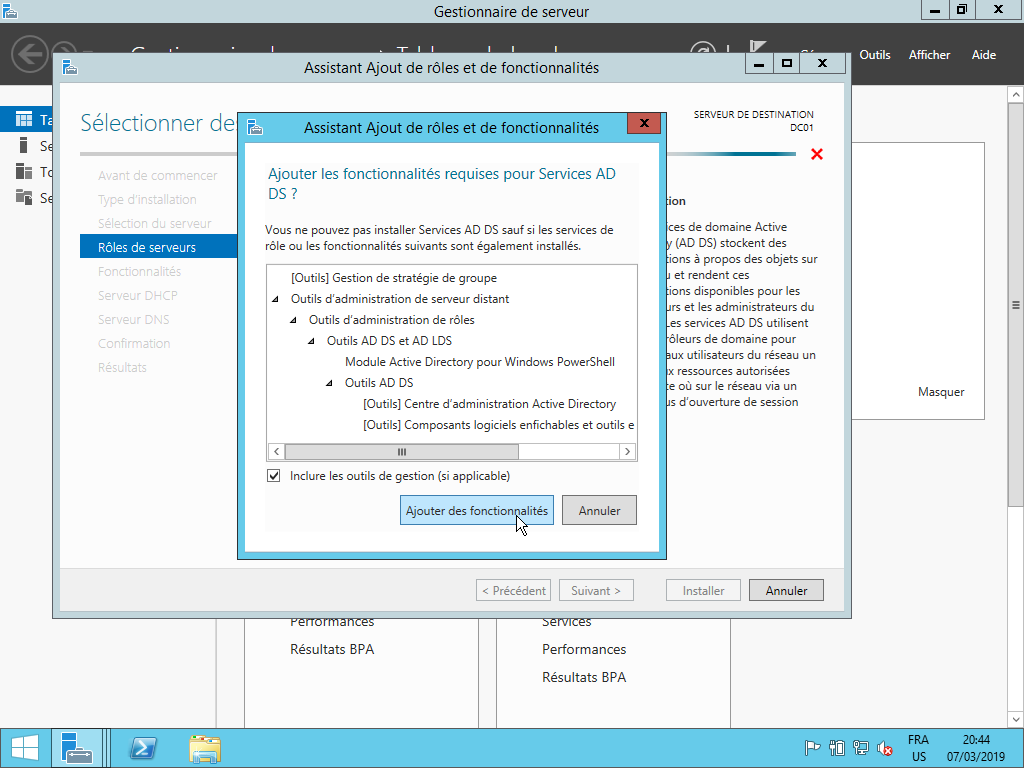
\includegraphics[scale=0.6]{WS2012_Screenshots/23.png}
        \caption{Ajout de AD DS - Assistant d'ajout de rôles et de fonctionnalités de Windows Server 2012}
        \label{WS2012_Screenshots/23}
    \end{center}
\end{figure}
\FloatBarrier

\newpage
Cliquer sur \textit{Ajouter des fonctionnalités} :
\begin{figure}[h!]
    \begin{center}
        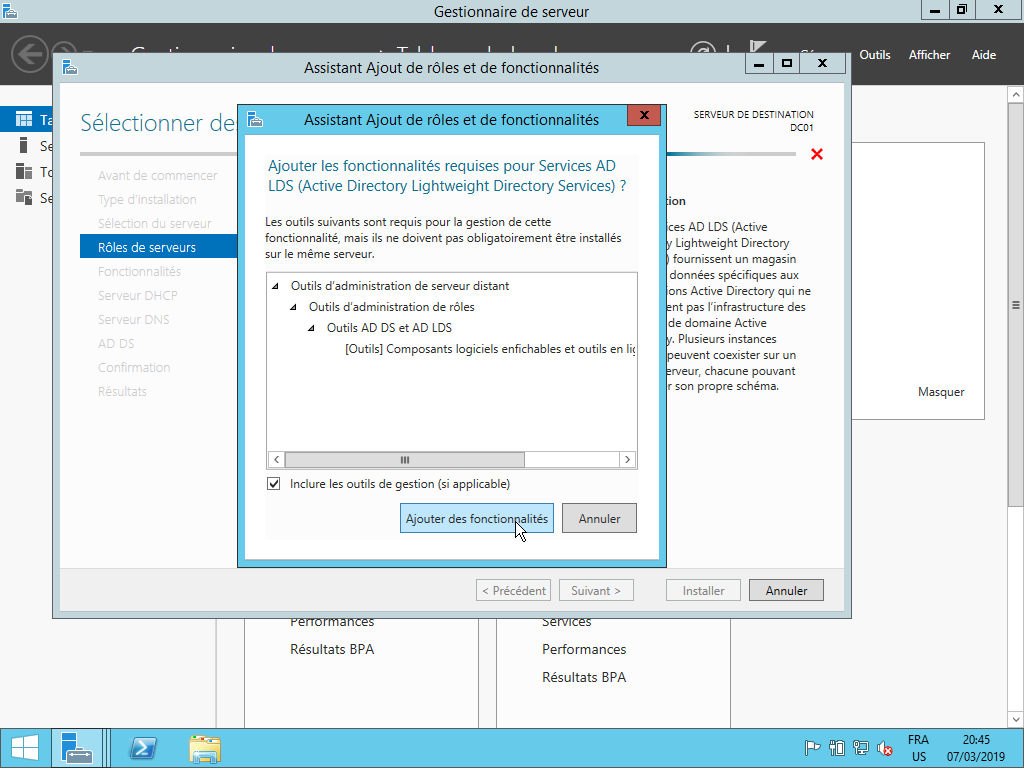
\includegraphics[scale=0.6]{WS2012_Screenshots/24.png}
        \caption{Ajout de AD LDS - Assistant d'ajout de rôles et de fonctionnalités de Windows Server 2012}
        \label{WS2012_Screenshots/24}
    \end{center}
\end{figure}
\FloatBarrier

\newpage
Cliquer sur \textit{Suivant} :
\begin{figure}[h!]
    \begin{center}
        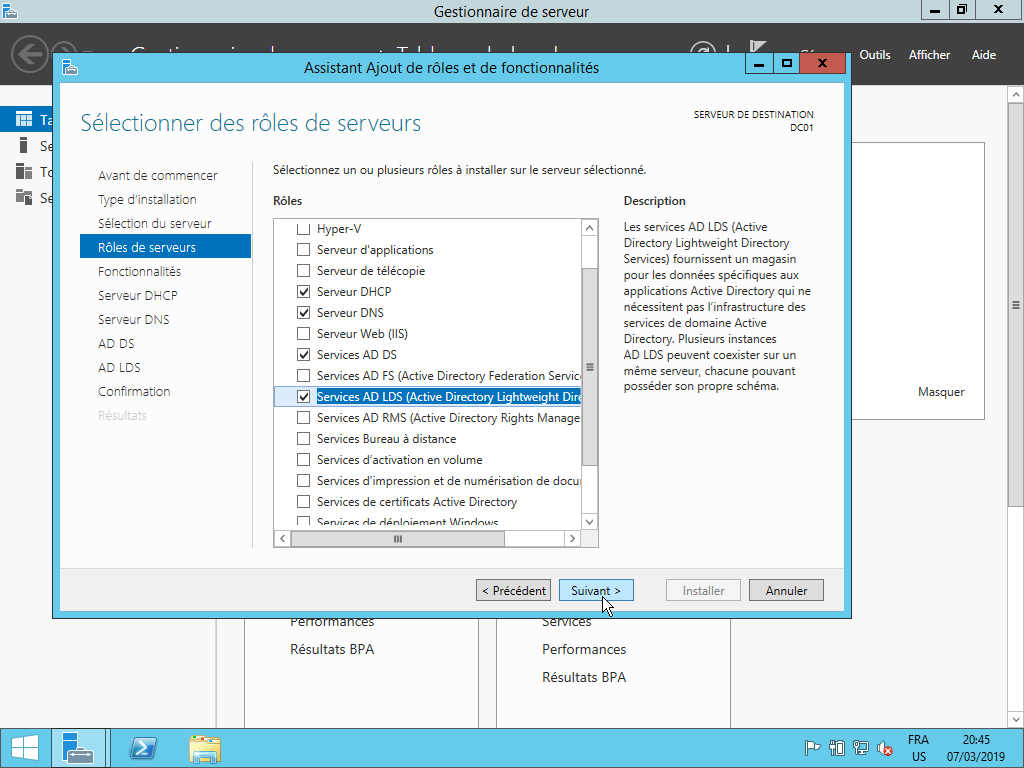
\includegraphics[scale=0.6]{WS2012_Screenshots/25.png}
        \caption{Etat des ajouts - Assistant d'ajout de rôles et de fonctionnalités de Windows Server 2012}
        \label{WS2012_Screenshots/25}
    \end{center}
\end{figure}
\FloatBarrier

\newpage
Aller dans la section \textbf{Fonctionnalités}. Cocher l'option de chiffrement de lecteur BitLocker. Cliquer sur \textit{Ajouter des fonctionnalités} :
\begin{figure}[h!]
    \begin{center}
        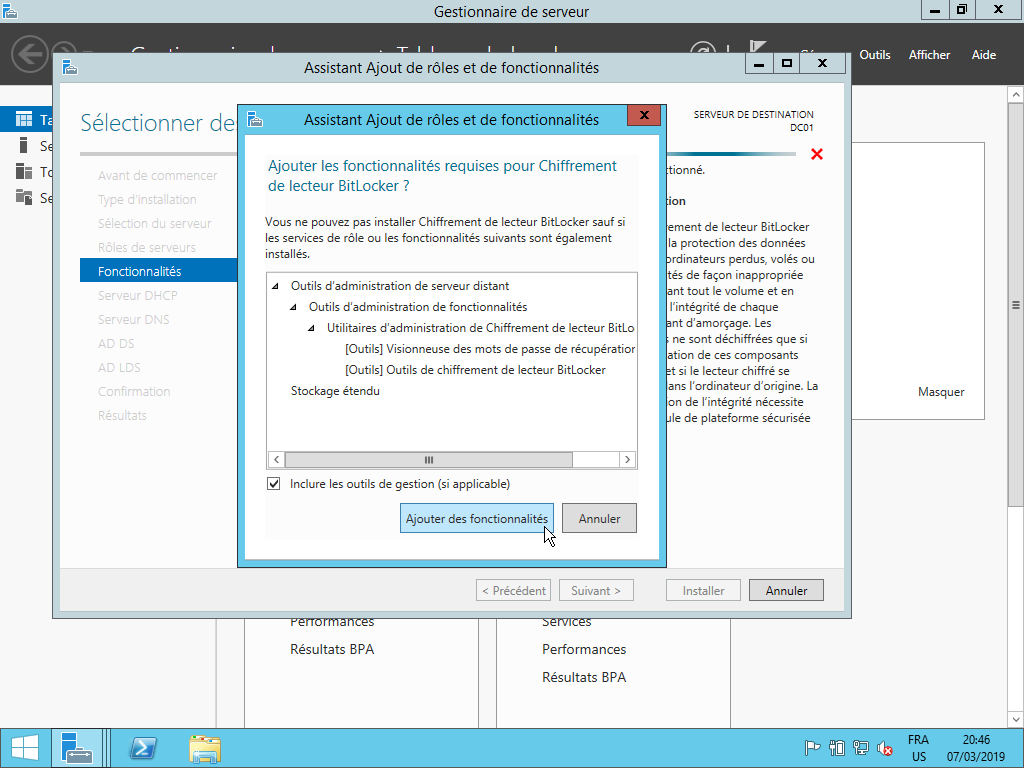
\includegraphics[scale=0.6]{WS2012_Screenshots/26.png}
        \caption{Ajout du chiffrement de lecteur BitLocker - Assistant d'ajout de rôles et de fonctionnalités de Windows Server 2012}
        \label{WS2012_Screenshots/26}
    \end{center}
\end{figure}
\FloatBarrier

\newpage
Aller dans la section \textbf{Serveur DHCP}. Cliquer sur \textit{Suivant} :
\begin{figure}[h!]
    \begin{center}
        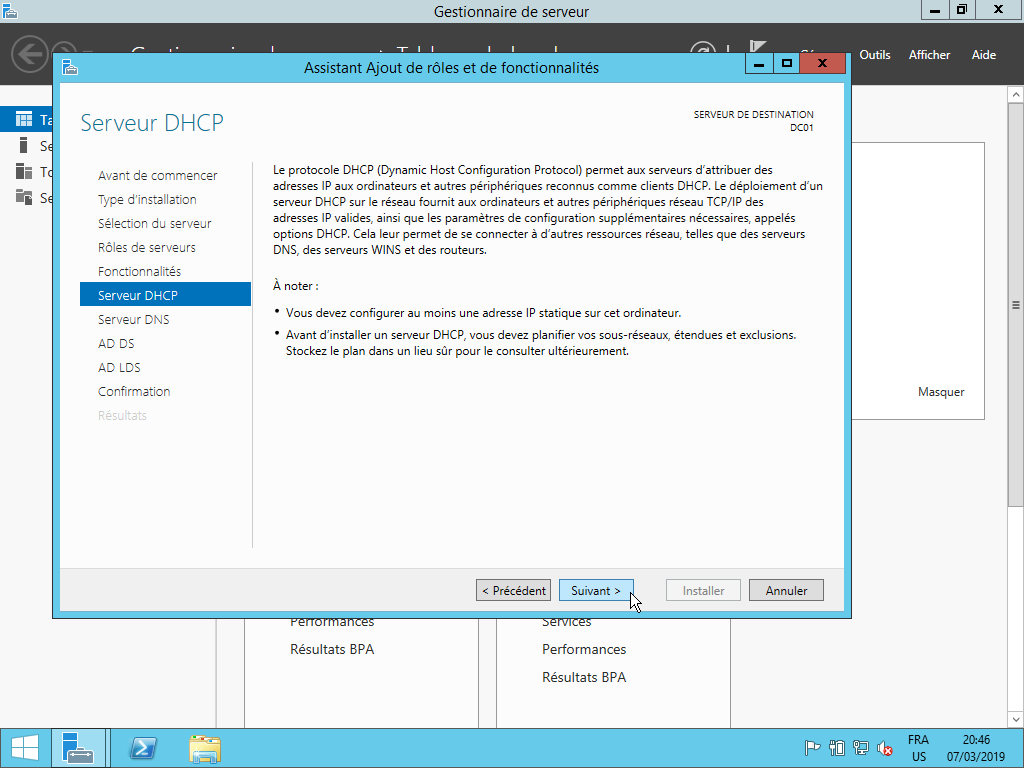
\includegraphics[scale=0.6]{WS2012_Screenshots/27.png}
        \caption{Finalisation DHCP - Assistant d'ajout de rôles et de fonctionnalités de Windows Server 2012}
        \label{WS2012_Screenshots/27}
    \end{center}
\end{figure}
\FloatBarrier

\newpage
Aller dans la section \textbf{Serveur DNS}. Cliquer sur \textit{Suivant} :
\begin{figure}[h!]
    \begin{center}
        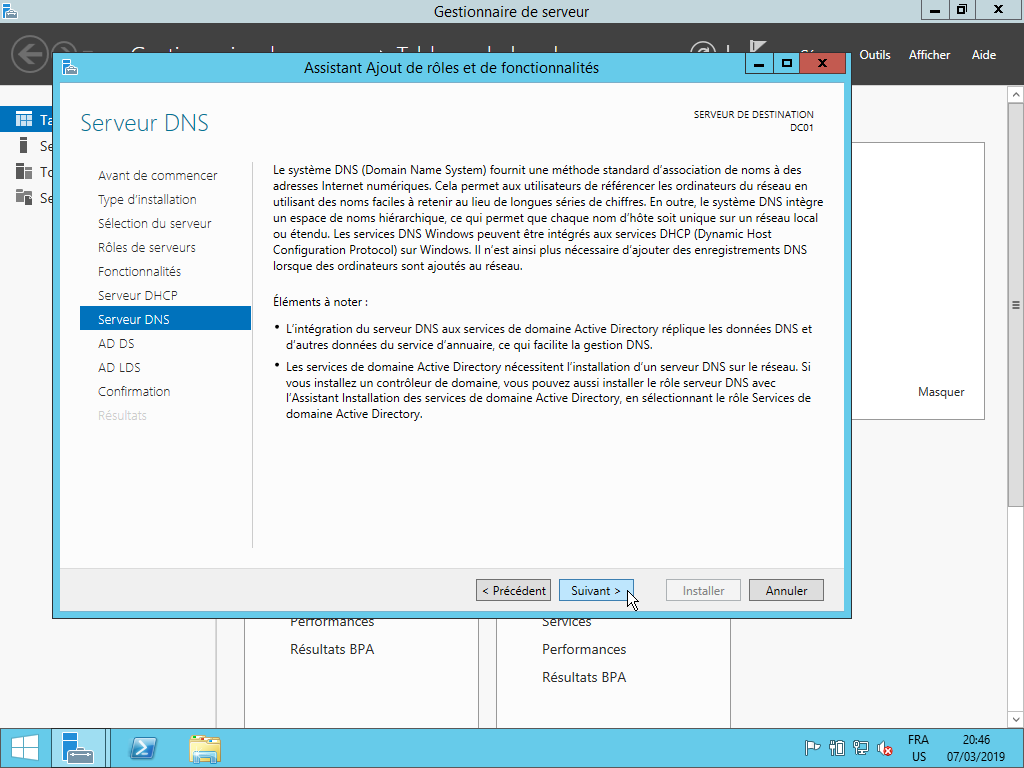
\includegraphics[scale=0.6]{WS2012_Screenshots/28.png}
        \caption{Finalisation DNS - Assistant d'ajout de rôles et de fonctionnalités de Windows Server 2012}
        \label{WS2012_Screenshots/28}
    \end{center}
\end{figure}
\FloatBarrier

\newpage
Aller dans la section \textbf{Serveur AD DS}. Cliquer sur \textit{Suivant} :
\begin{figure}[h!]
    \begin{center}
        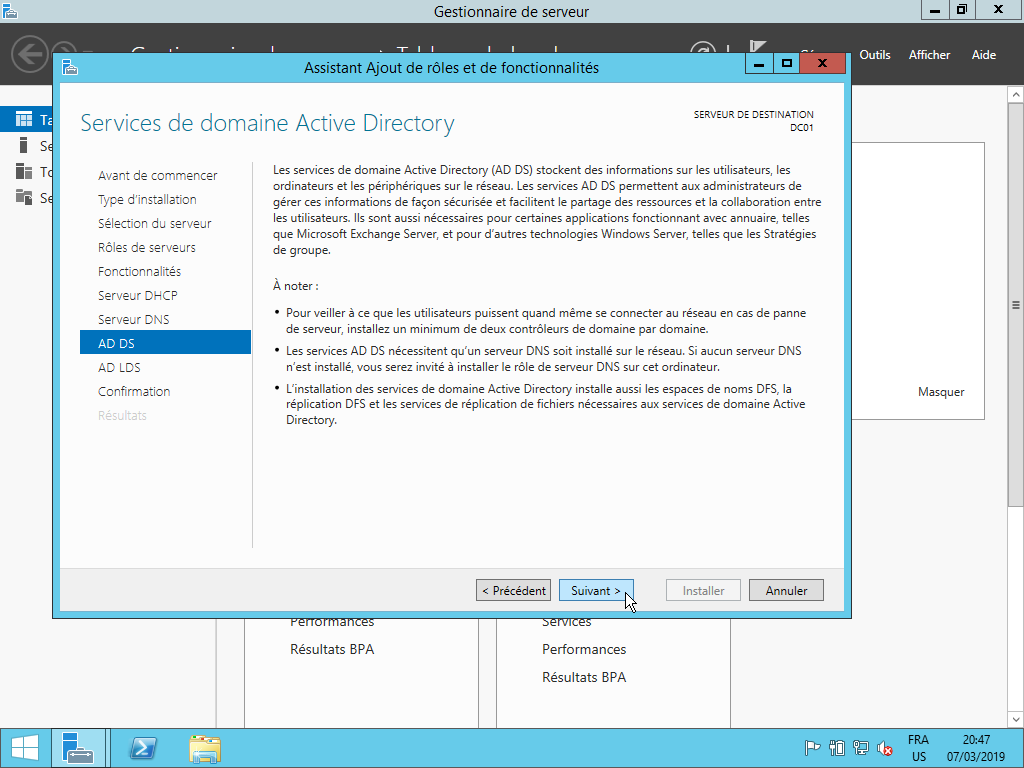
\includegraphics[scale=0.6]{WS2012_Screenshots/29.png}
        \caption{Finalisation AD DS - Assistant d'ajout de rôles et de fonctionnalités de Windows Server 2012}
        \label{WS2012_Screenshots/29}
    \end{center}
\end{figure}
\FloatBarrier

\newpage
Aller dans la section \textbf{Serveur AD LDS}. Cliquer sur \textit{Suivant} :
\begin{figure}[h!]
    \begin{center}
        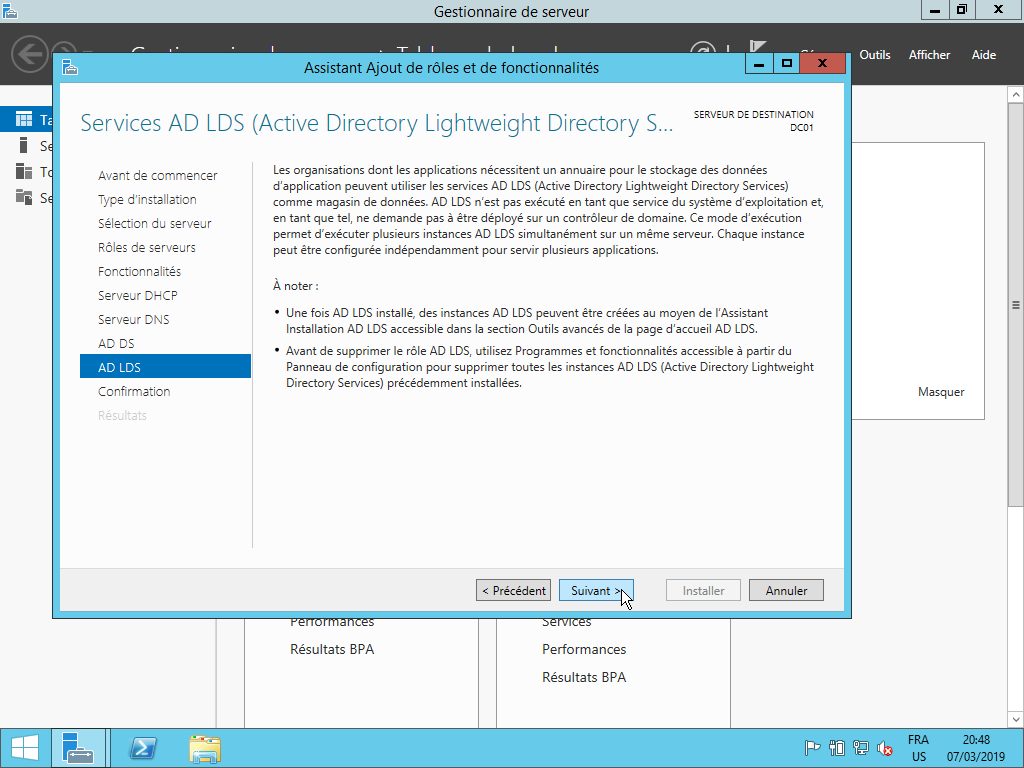
\includegraphics[scale=0.6]{WS2012_Screenshots/30.png}
        \caption{Finalisation AD LDS - Assistant d'ajout de rôles et de fonctionnalités de Windows Server 2012}
        \label{WS2012_Screenshots/30}
    \end{center}
\end{figure}
\FloatBarrier

\newpage
Aller dans la section \textbf{Confirmation}. Cliquer sur \textit{Installer} :
\begin{figure}[h!]
    \begin{center}
        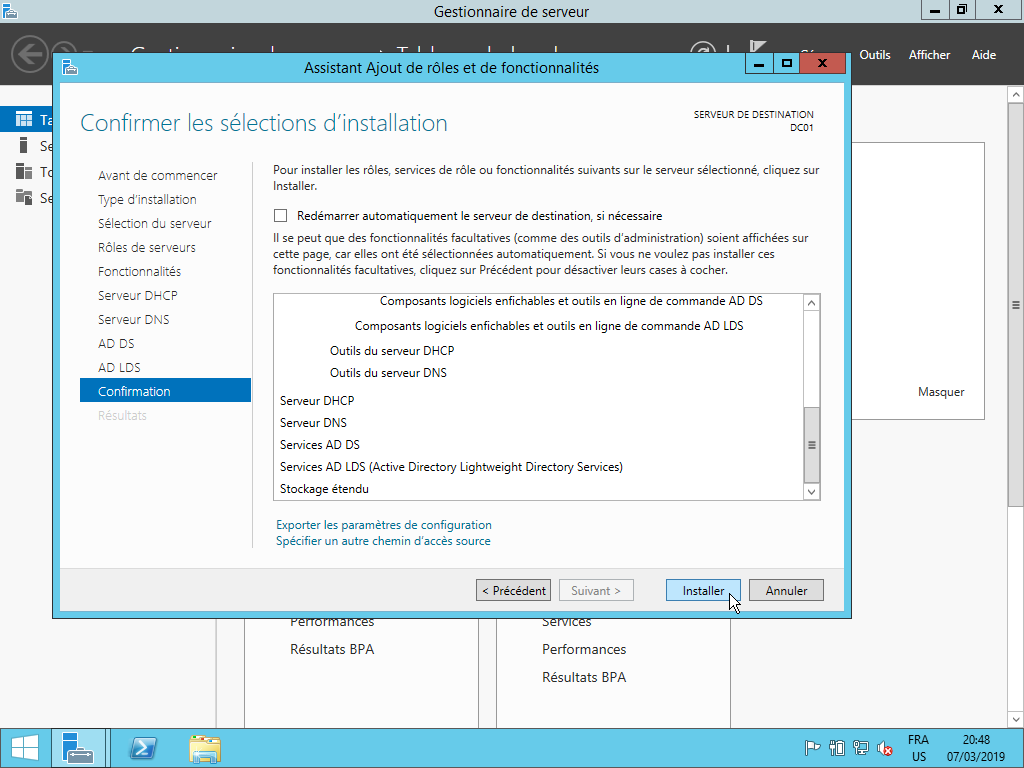
\includegraphics[scale=0.6]{WS2012_Screenshots/31.png}
        \caption{Confirmation des sélections - Assistant d'ajout de rôles et de fonctionnalités de Windows Server 2012}
        \label{WS2012_Screenshots/31}
    \end{center}
\end{figure}
\FloatBarrier

\newpage
Aller dans la section \textbf{Résultats}, et attendre la fin de l'installation :
\begin{figure}[h!]
    \begin{center}
        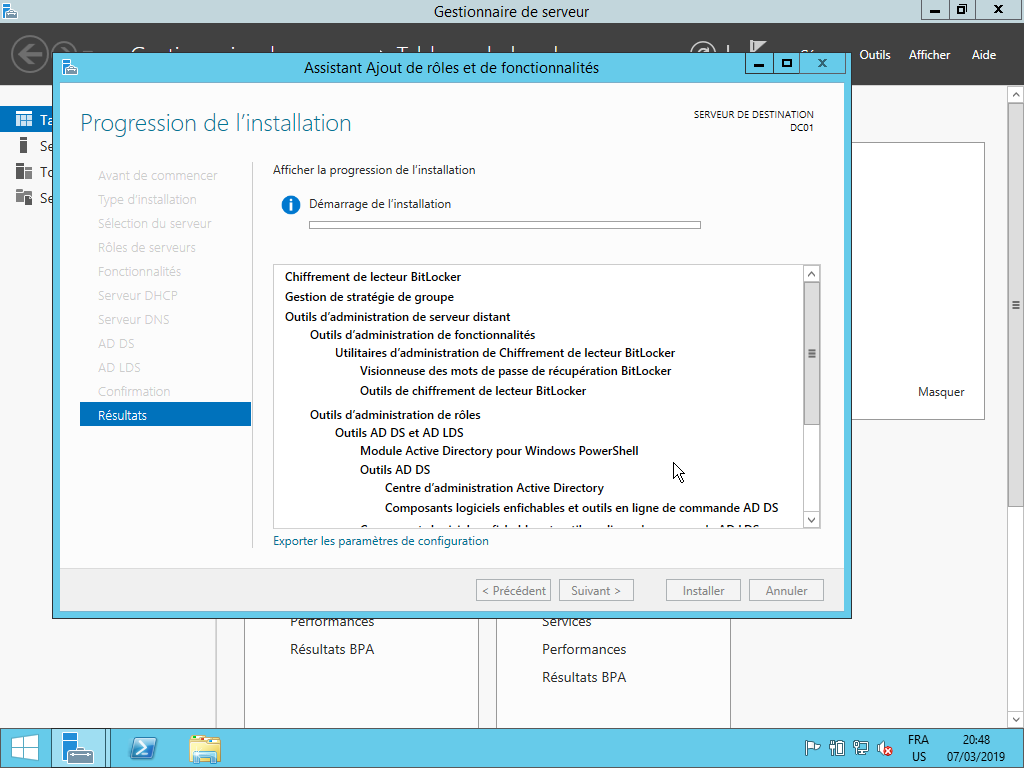
\includegraphics[scale=0.6]{WS2012_Screenshots/32.png}
        \caption{Installation - Assistant d'ajout de rôles et de fonctionnalités de Windows Server 2012}
        \label{WS2012_Screenshots/32}
    \end{center}
\end{figure}
\FloatBarrier

\newpage
Fin de l'installation. Cliquer sur \textit{Fermer} :
\begin{figure}[h!]
    \begin{center}
        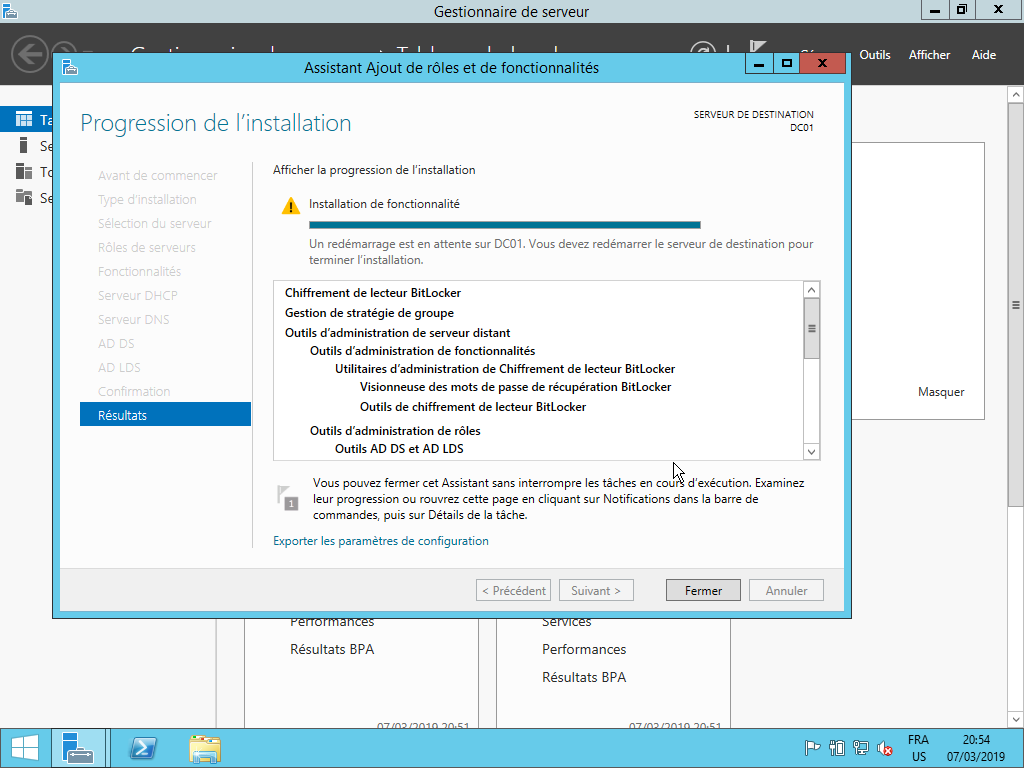
\includegraphics[scale=0.6]{WS2012_Screenshots/33.png}
        \caption{Fin de l'installation - Assistant d'ajout de rôles et de fonctionnalités de Windows Server 2012}
        \label{WS2012_Screenshots/33}
    \end{center}
\end{figure}
\FloatBarrier

\newpage
\subsection{Configuration du DNS}

Cliquer sur \textit{Outils}, puis cliquer sur DNS :
\begin{figure}[h!]
    \begin{center}
        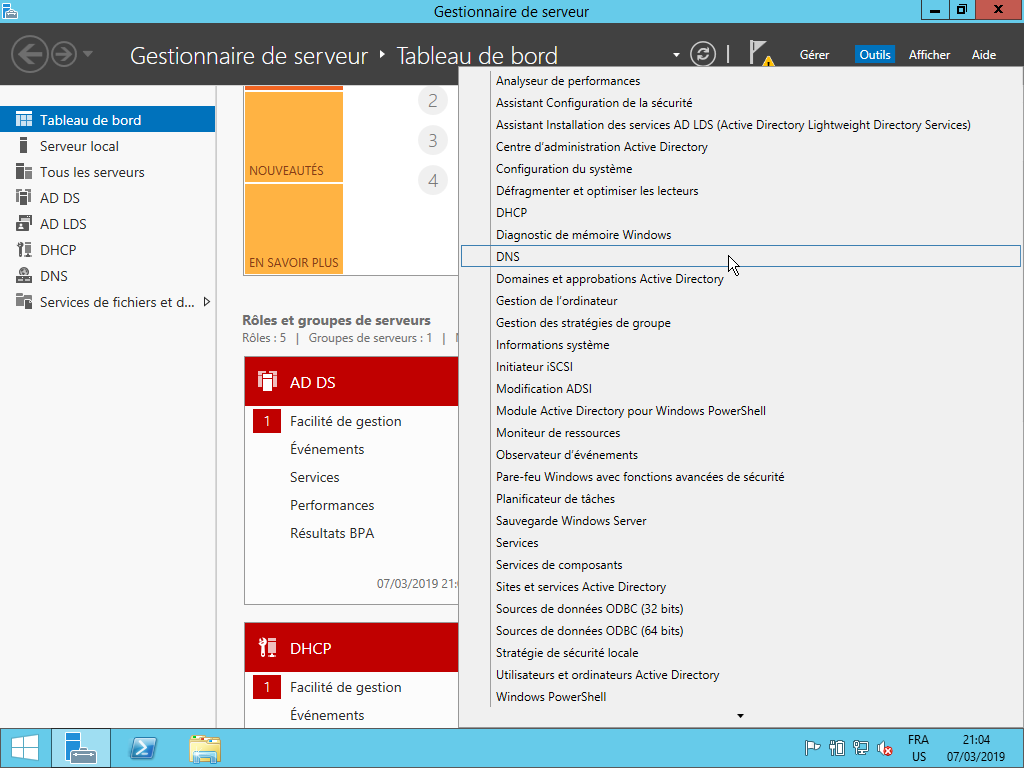
\includegraphics[scale=0.6]{WS2012_Screenshots/34.png}
        \caption{Accès au gestionnaire DNS de Windows Server 2012}
        \label{WS2012_Screenshots/34}
    \end{center}
\end{figure}
\FloatBarrier

\newpage
Cliquer droit sur \texttt{Redirecteurs}, puis cliquer sur \textit{Propriétés} :
\begin{figure}[h!]
    \begin{center}
        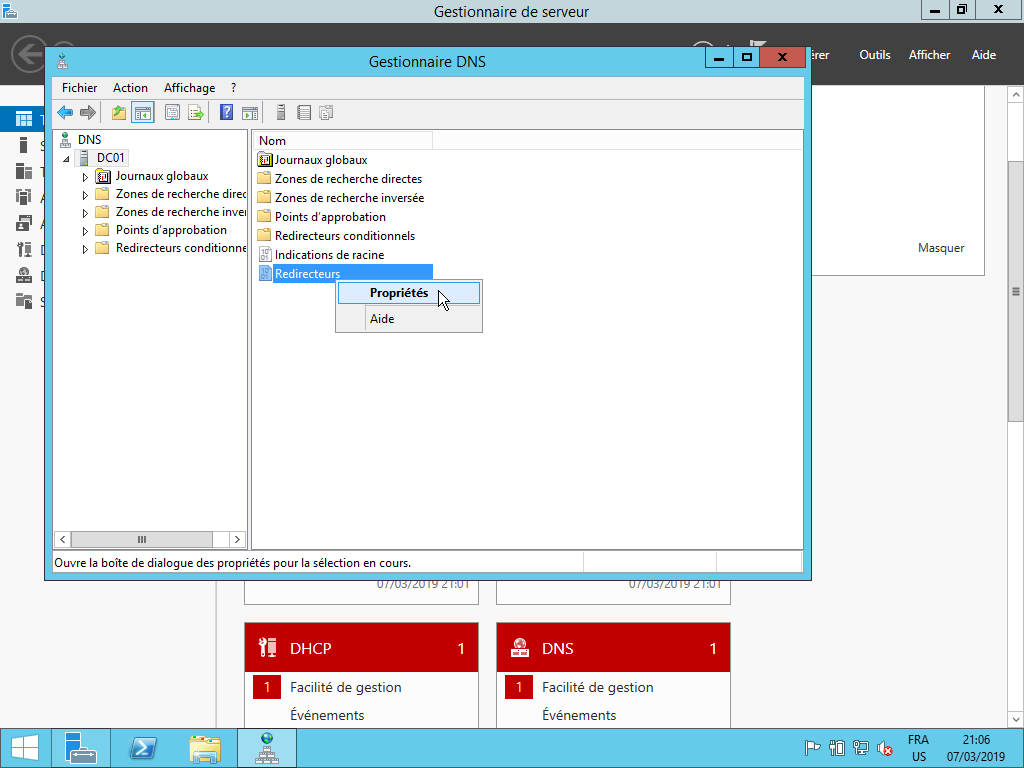
\includegraphics[scale=0.6]{WS2012_Screenshots/35.png}
        \caption{Accès aux propriétés des Redirecteurs - Gestionnaire DNS de Windows Server 2012}
        \label{WS2012_Screenshots/35}
    \end{center}
\end{figure}
\FloatBarrier

\newpage
Entrer la valeur "8.8.8.8" dans le nouveau champ :
\begin{figure}[h!]
    \begin{center}
        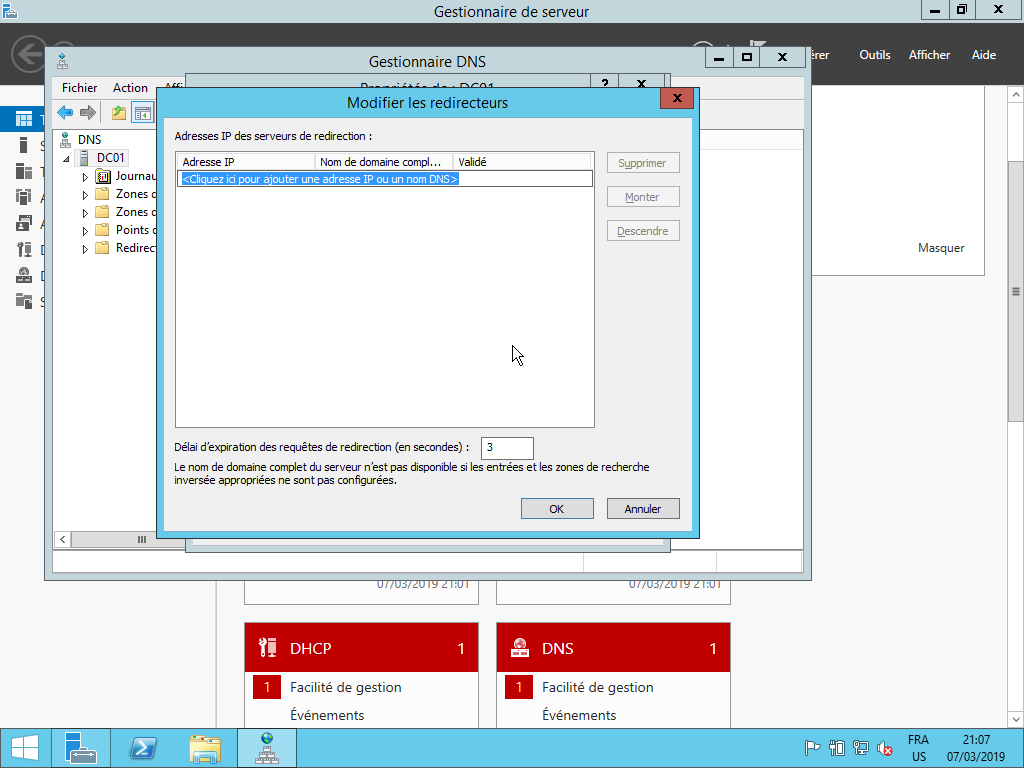
\includegraphics[scale=0.6]{WS2012_Screenshots/36.png}
        \caption{Ajout d'une valeur dans les Redirecteurs - Gestionnaire DNS de Windows Server 2012}
        \label{WS2012_Screenshots/36}
    \end{center}
\end{figure}
\FloatBarrier

\newpage
Cliquer sur \textit{OK} :
\begin{figure}[h!]
    \begin{center}
        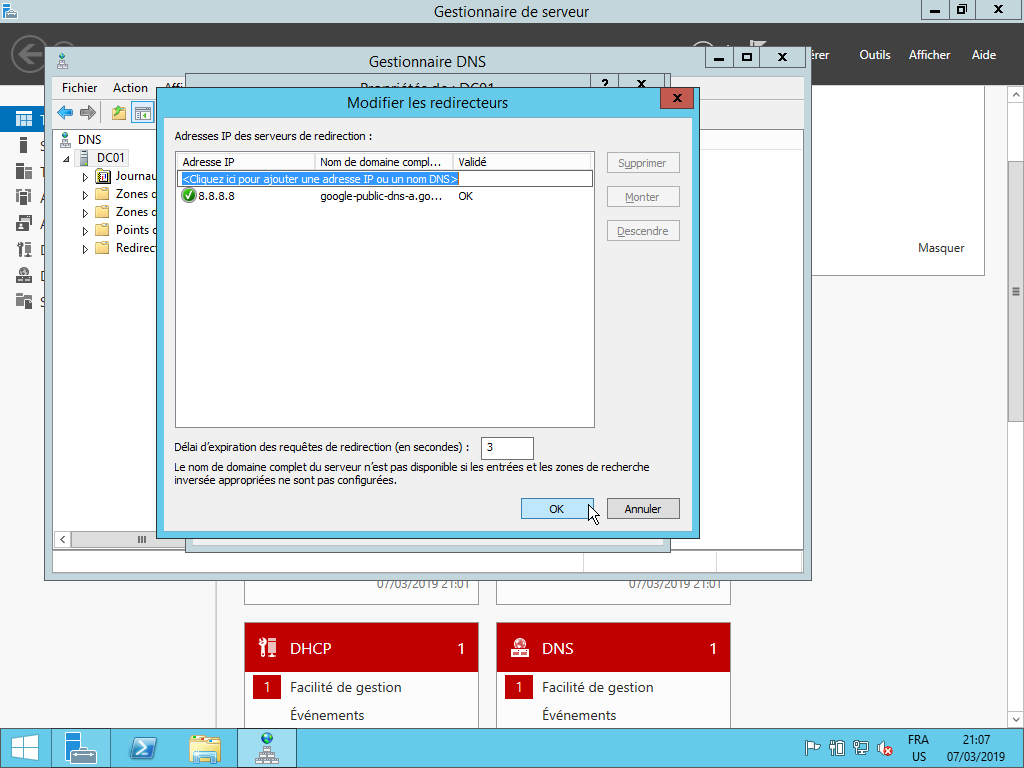
\includegraphics[scale=0.6]{WS2012_Screenshots/37.png}
        \caption{Vérification de la valeur dans les Redirecteurs - Gestionnaire DNS de Windows Server 2012}
        \label{WS2012_Screenshots/37}
    \end{center}
\end{figure}
\FloatBarrier

\newpage
Cocher l'option "\textit{Ce serveur assure la maintenance de la zone}", puis cliquer sur \textit{Suivant} :
\begin{figure}[h!]
    \begin{center}
        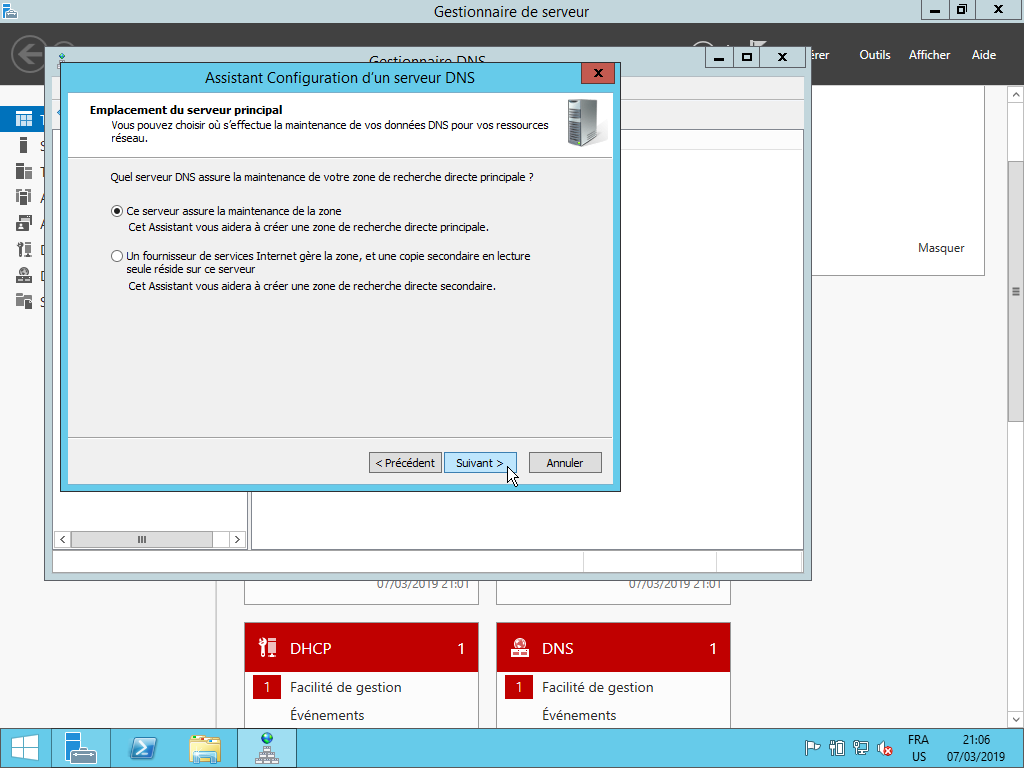
\includegraphics[scale=0.6]{WS2012_Screenshots/38.png}
        \caption{Assistant configuration d'un serveur DNS - Gestionnaire DNS de Windows Server 2012}
        \label{WS2012_Screenshots/38}
    \end{center}
\end{figure}
\FloatBarrier

\newpage
Cliquer sur \textit{Appliquer} :
\begin{figure}[h!]
    \begin{center}
        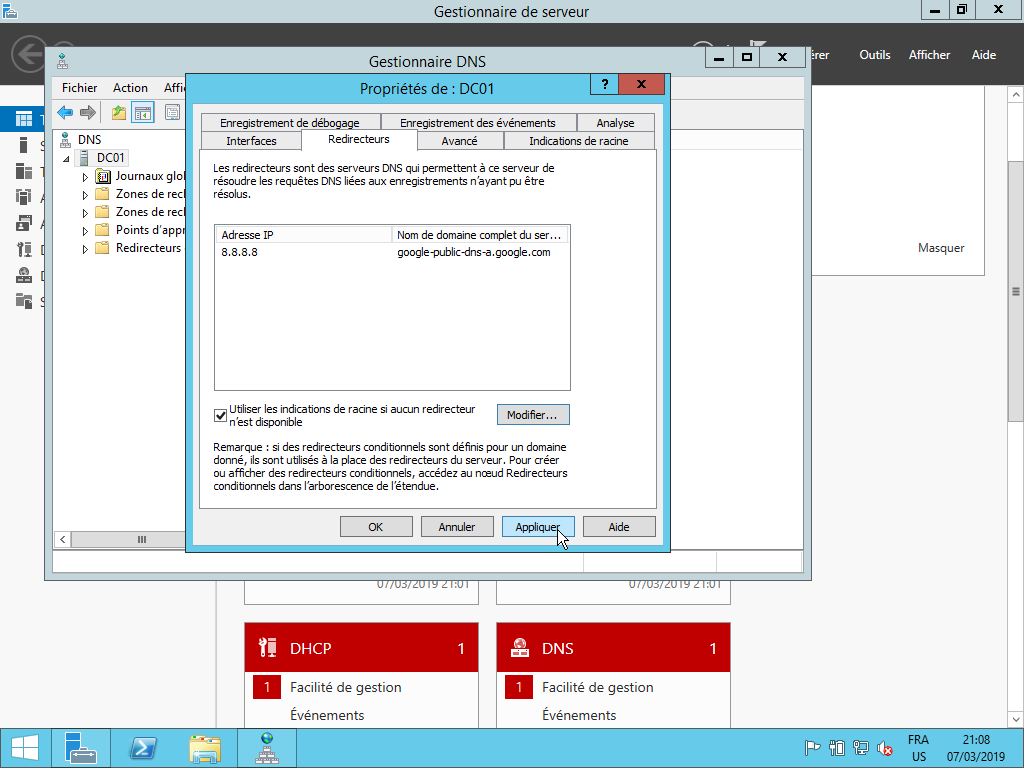
\includegraphics[scale=0.5]{WS2012_Screenshots/39.png}
        \caption{Application du paramétrage des Redirecteurs - Gestionnaire DNS de Windows Server 2012}
        \label{WS2012_Screenshots/39}
    \end{center}
\end{figure}
\FloatBarrier

\newpage
\subsection{Gestion du DHCP}

Cliquer sur \textit{Outils}, puis cliquer sur DHCP :
\begin{figure}[h!]
    \begin{center}
        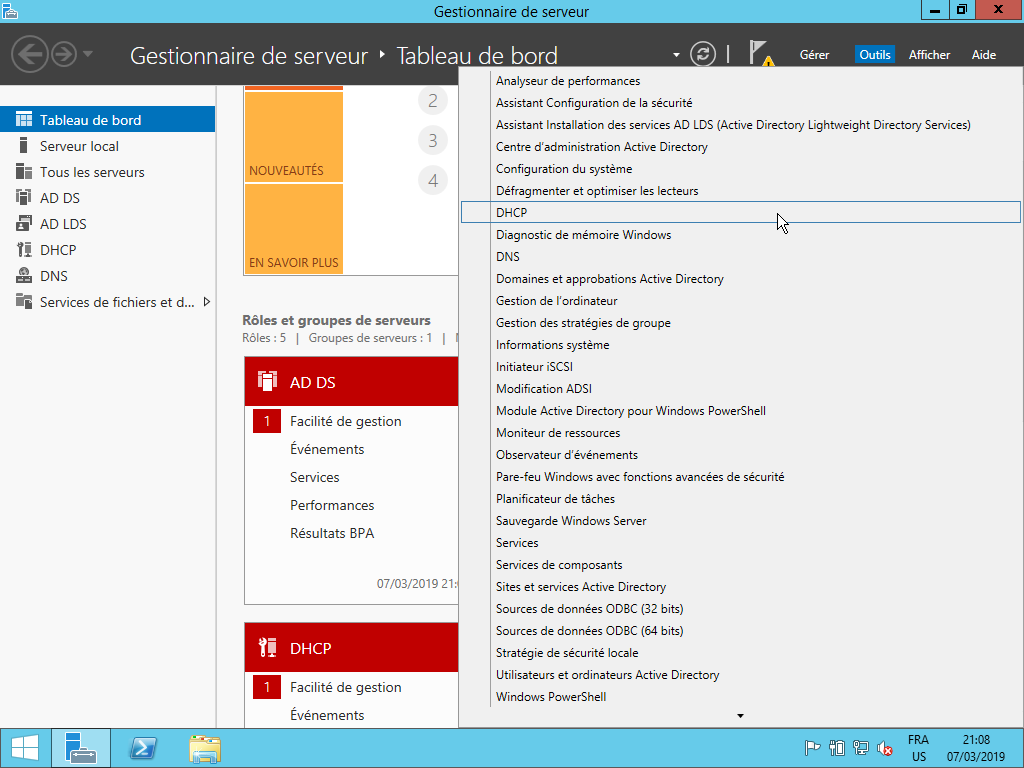
\includegraphics[scale=0.6]{WS2012_Screenshots/40.png}
        \caption{Accès au gestionnaire DHCP de Windows Server 2012}
        \label{WS2012_Screenshots/40}
    \end{center}
\end{figure}
\FloatBarrier

\newpage
Cliquer droit sur IPv4, puis cliquer sur \textit{Propriétés} :
\begin{figure}[h!]
    \begin{center}
        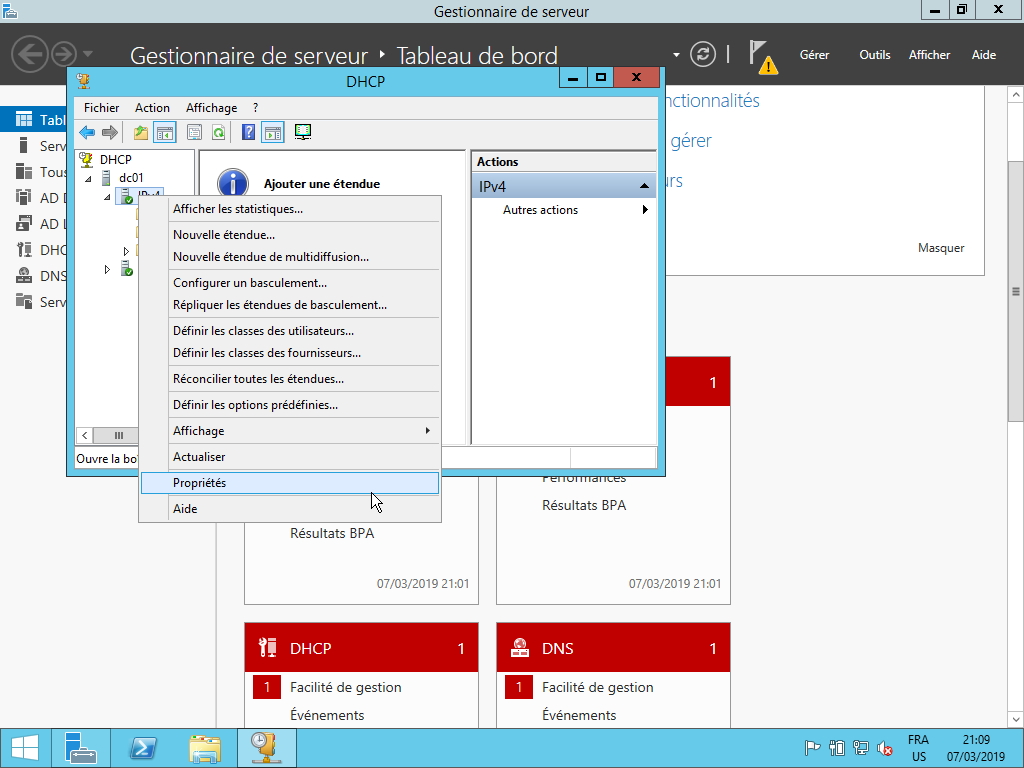
\includegraphics[scale=0.6]{WS2012_Screenshots/41.png}
        \caption{Nouvelle étendue DHCP sur IPv4 - Gestionnaire DHCP de Windows Server 2012}
        \label{WS2012_Screenshots/41}
    \end{center}
\end{figure}
\FloatBarrier

\newpage
Cliquer sur \textit{Suivant} :
\begin{figure}[h!]
    \begin{center}
        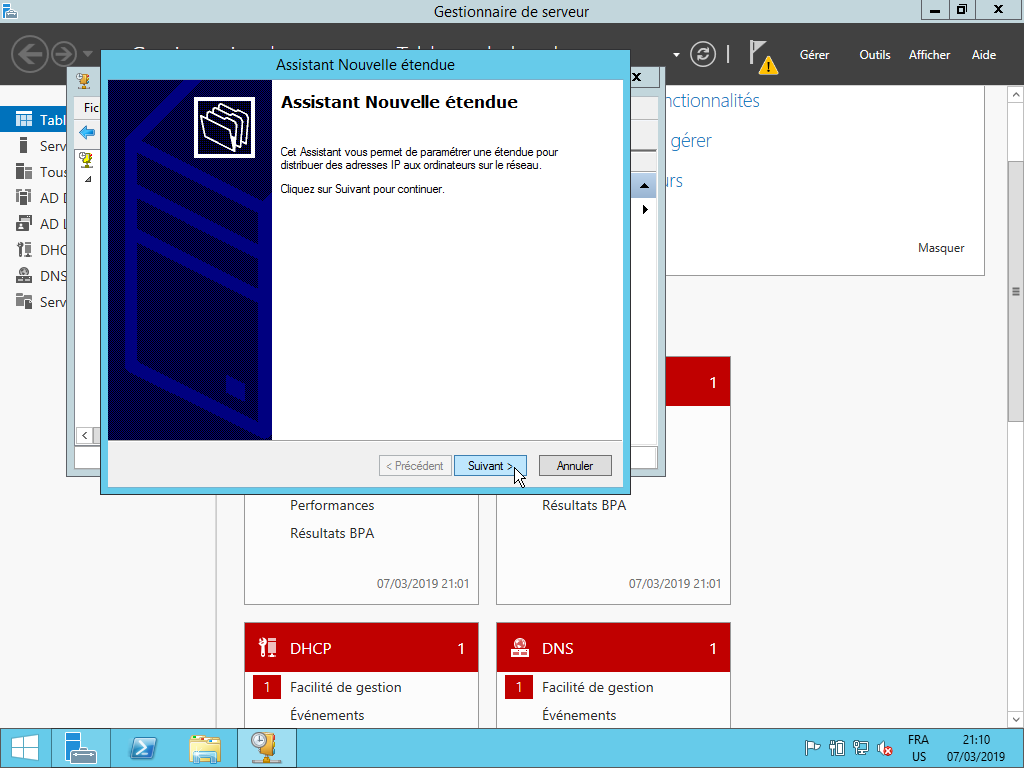
\includegraphics[scale=0.6]{WS2012_Screenshots/42.png}
        \caption{Assistant Nouvelle étendue - Gestionnaire DHCP de Windows Server 2012}
        \label{WS2012_Screenshots/42}
    \end{center}
\end{figure}
\FloatBarrier

\newpage
Entrer la valeur "Etendu EPITAF" dans le champ \textit{Nom}, et "192.168.2.10-192.168.2.20" dans le champ \textit{Description}. Cliquer sur \textit{Suivant} :
\begin{figure}[h!]
    \begin{center}
        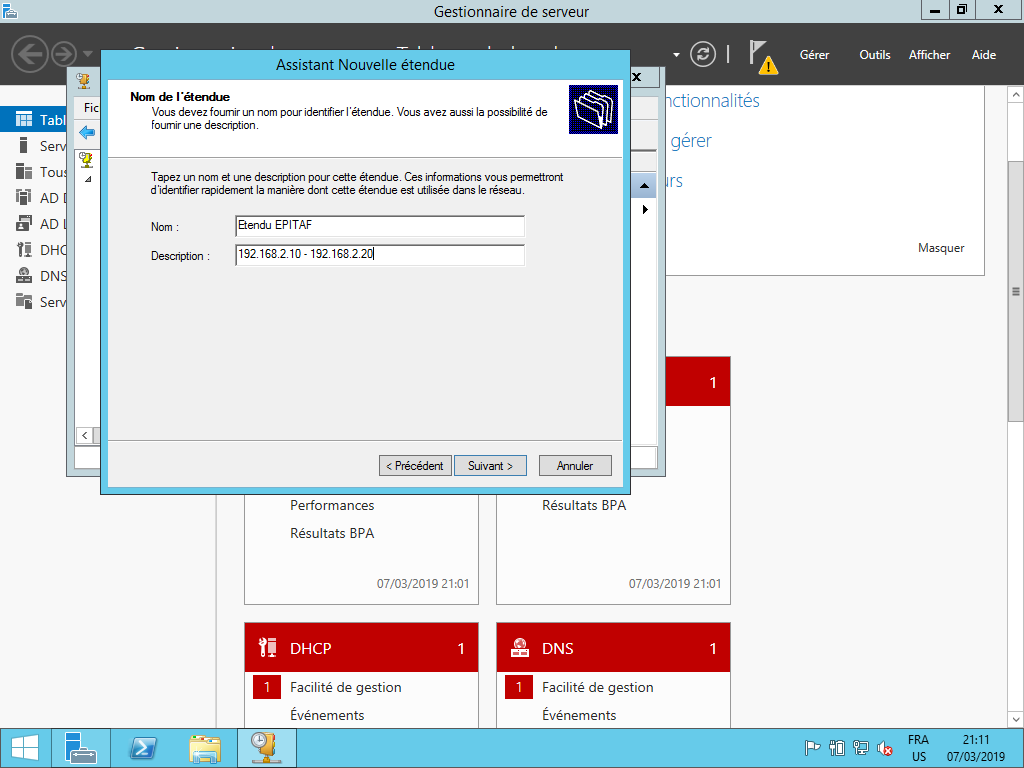
\includegraphics[scale=0.6]{WS2012_Screenshots/43.png}
        \caption{Nom et description - Assistant Nouvelle étendue du Gestionnaire DHCP de Windows Server 2012}
        \label{WS2012_Screenshots/43}
    \end{center}
\end{figure}
\FloatBarrier

\newpage
Entrer les valeurs suivantes :
\begin{itemize}
    \item Adresse IP de début : 192.168.2.10
    \item Adresse IP de fin : 192.168.2.20
    \item Longueur : 24
    \item Masque de sous-réseau : 255.255.255.0
\end{itemize}
Cliquer sur \textit{Suivant} :
\begin{figure}[h!]
    \begin{center}
        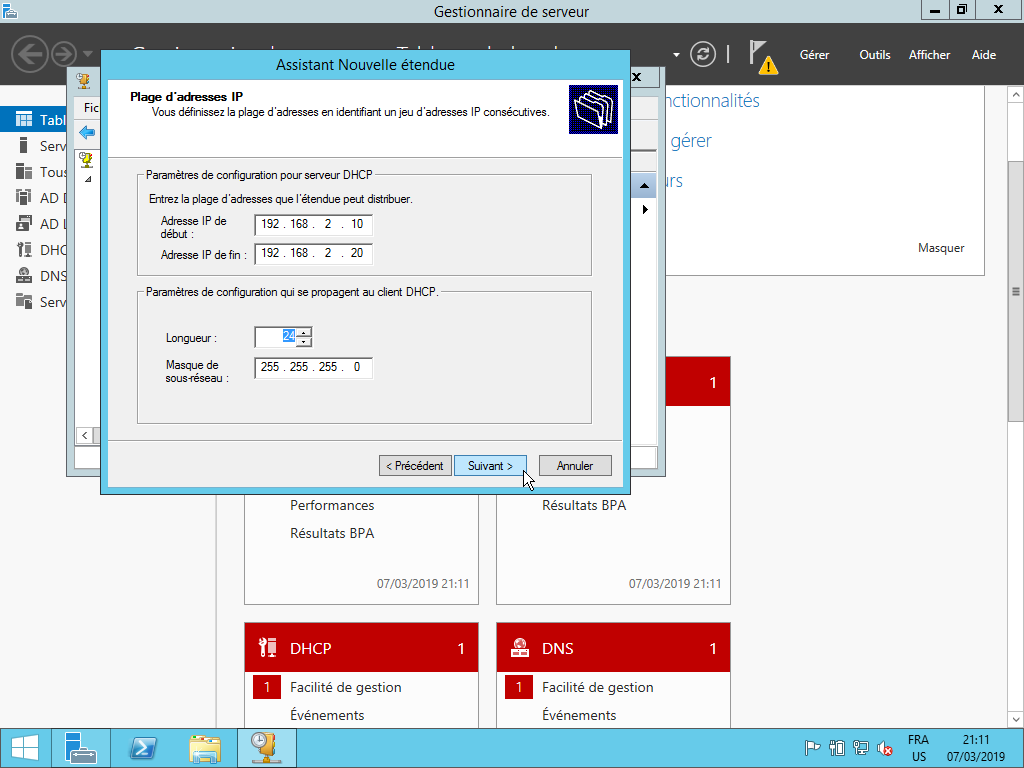
\includegraphics[scale=0.6]{WS2012_Screenshots/44.png}
        \caption{Plage d'adresses IP - Assistant Nouvelle étendue du Gestionnaire DHCP de Windows Server 2012}
        \label{WS2012_Screenshots/44}
    \end{center}
\end{figure}
\FloatBarrier

\newpage
Cliquer sur \textit{Suivant} :
\begin{figure}[h!]
    \begin{center}
        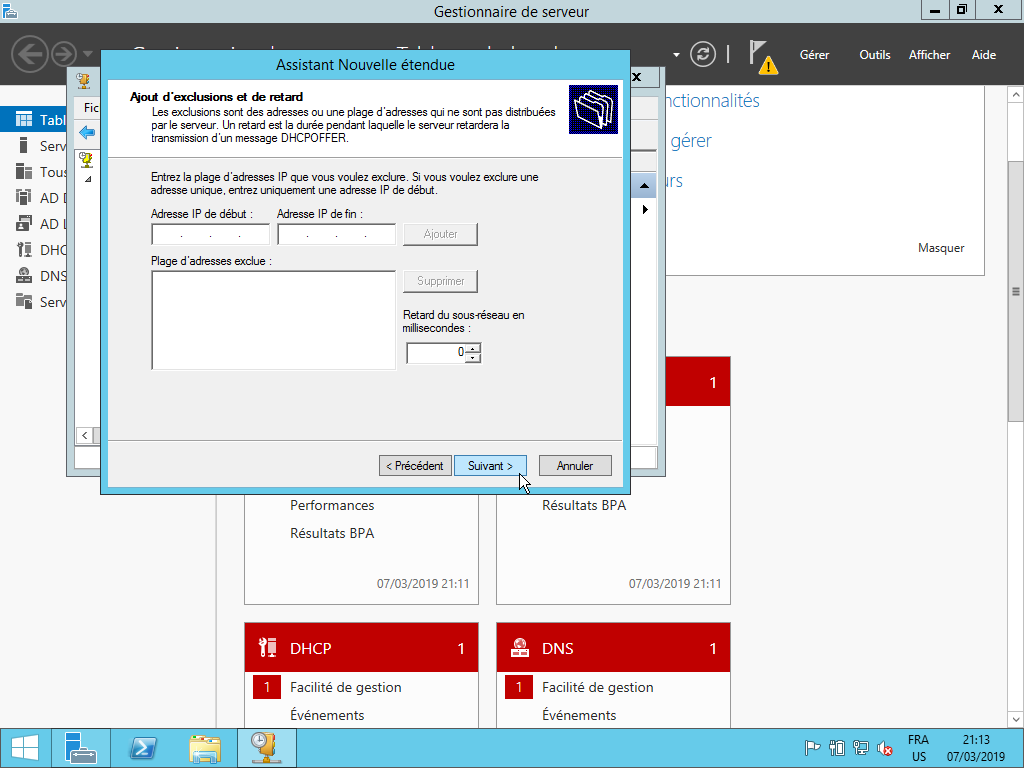
\includegraphics[scale=0.6]{WS2012_Screenshots/45.png}
        \caption{Ajout d'exclusions et de retard - Assistant Nouvelle étendue du Gestionnaire DHCP de Windows Server 2012}
        \label{WS2012_Screenshots/45}
    \end{center}
\end{figure}
\FloatBarrier

\newpage
Cliquer sur \textit{Suivant} :
\begin{figure}[h!]
    \begin{center}
        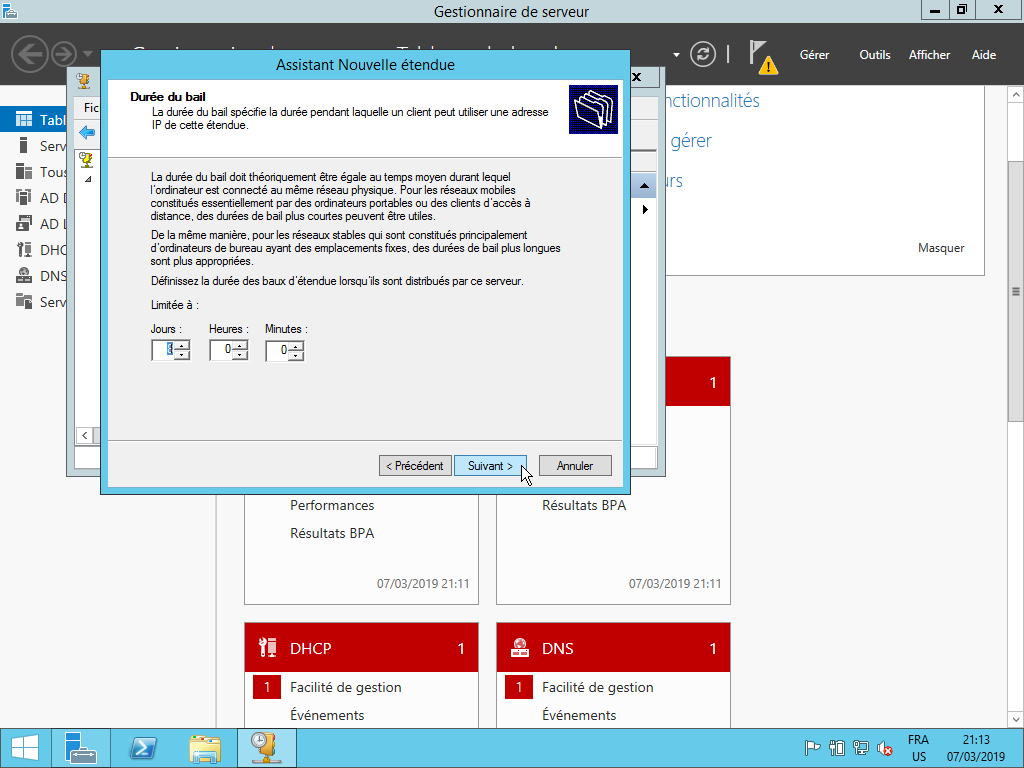
\includegraphics[scale=0.6]{WS2012_Screenshots/46.png}
        \caption{Durée du bail - Assistant Nouvelle étendue du Gestionnaire DHCP de Windows Server 2012}
        \label{WS2012_Screenshots/46}
    \end{center}
\end{figure}
\FloatBarrier

\newpage
Cocher l'option "\textit{Oui, je veux configurer ces options maintenant}", et cliquer sur \textit{Suivant} :
\begin{figure}[h!]
    \begin{center}
        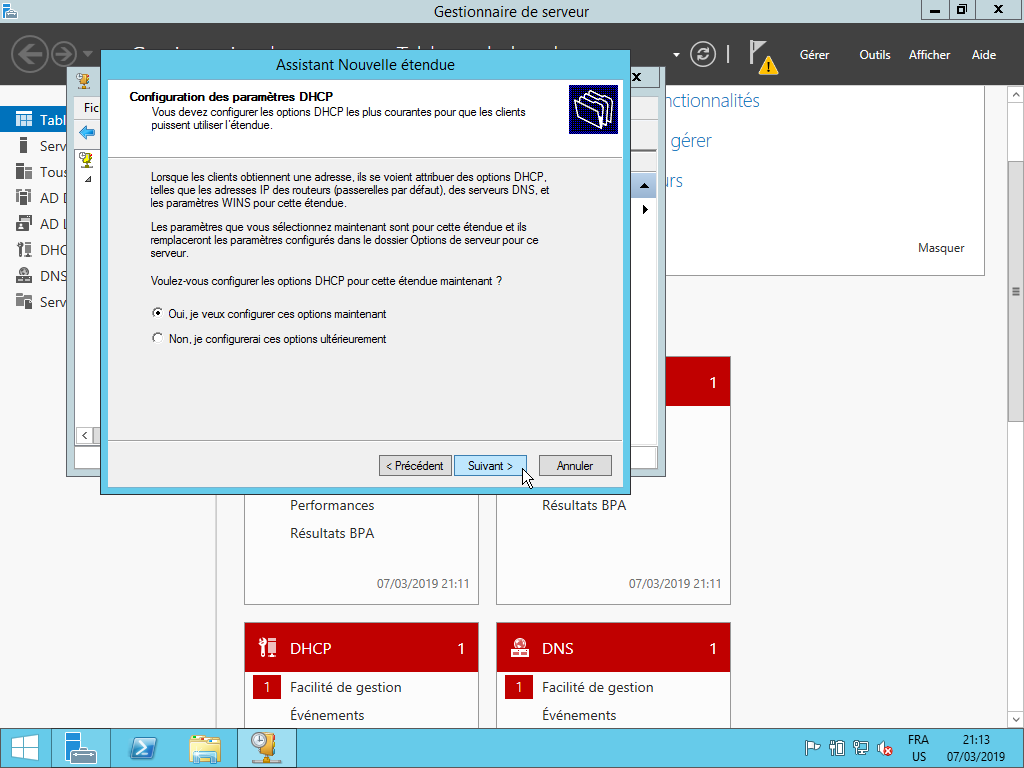
\includegraphics[scale=0.6]{WS2012_Screenshots/47.png}
        \caption{Configuration des paramètres DHCP - Assistant Nouvelle étendue du Gestionnaire DHCP de Windows Server 2012}
        \label{WS2012_Screenshots/47}
    \end{center}
\end{figure}
\FloatBarrier

\newpage
Entrer l'adresse IP 192.168.2.1, puis cliquer sur \textit{Ajouter}. Ensuite, cliquer sur \textit{Suivant} :
\begin{figure}[h!]
    \begin{center}
        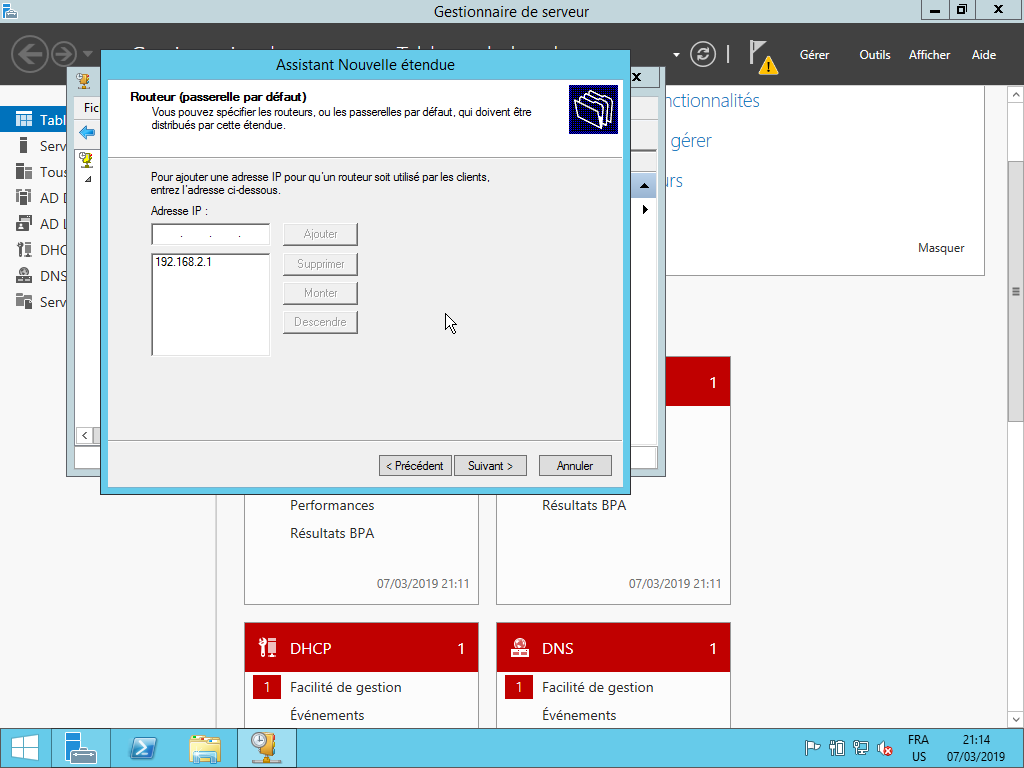
\includegraphics[scale=0.6]{WS2012_Screenshots/48.png}
        \caption{Routeur - Assistant Nouvelle étendue du Gestionnaire DHCP de Windows Server 2012}
        \label{WS2012_Screenshots/48}
    \end{center}
\end{figure}
\FloatBarrier

\newpage
Remplir les champs comme sur la figure suivante :
\begin{itemize}
    \item Domaine parent : EPITAF
    \item Nom du serveur : Controleur de domain
    \item Adresse IP : 192.168.2.2 et 8.8.8.8
\end{itemize}
Cliquer sur \textit{Suivant} :
\begin{figure}[h!]
    \begin{center}
        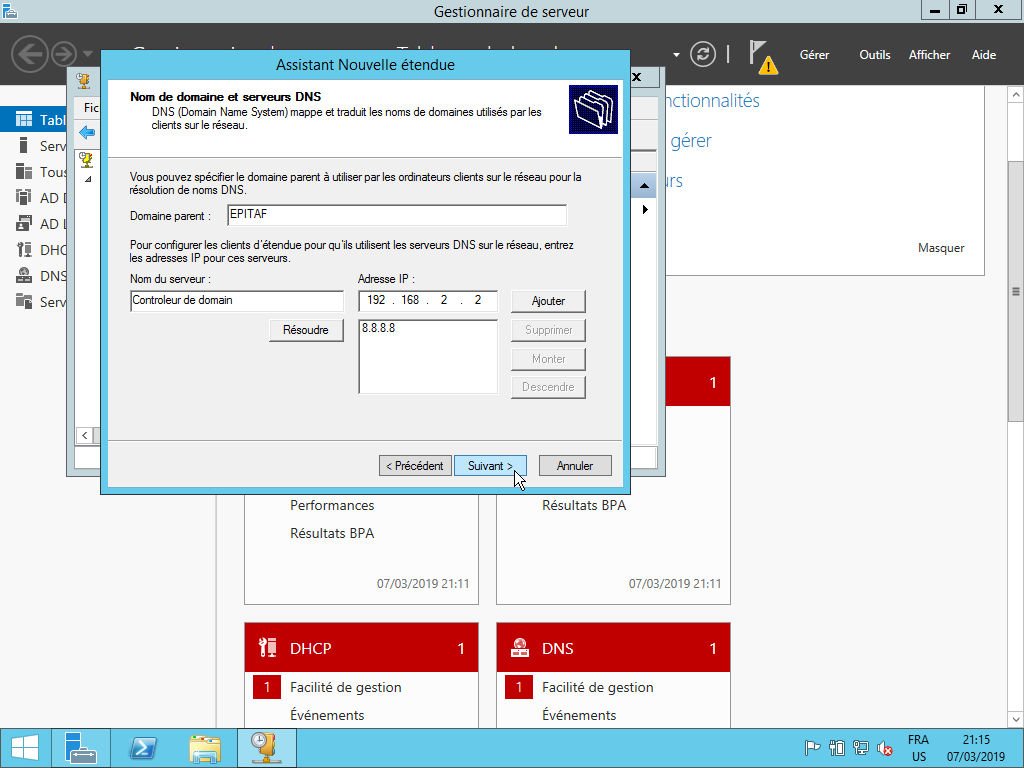
\includegraphics[scale=0.6]{WS2012_Screenshots/49.png}
        \caption{Nom de domaine et serveurs DNS - Assistant Nouvelle étendue du Gestionnaire DHCP de Windows Server 2012}
        \label{WS2012_Screenshots/49}
    \end{center}
\end{figure}
\FloatBarrier

\newpage
Cliquer sur \textit{Suivant} :
\begin{figure}[h!]
    \begin{center}
        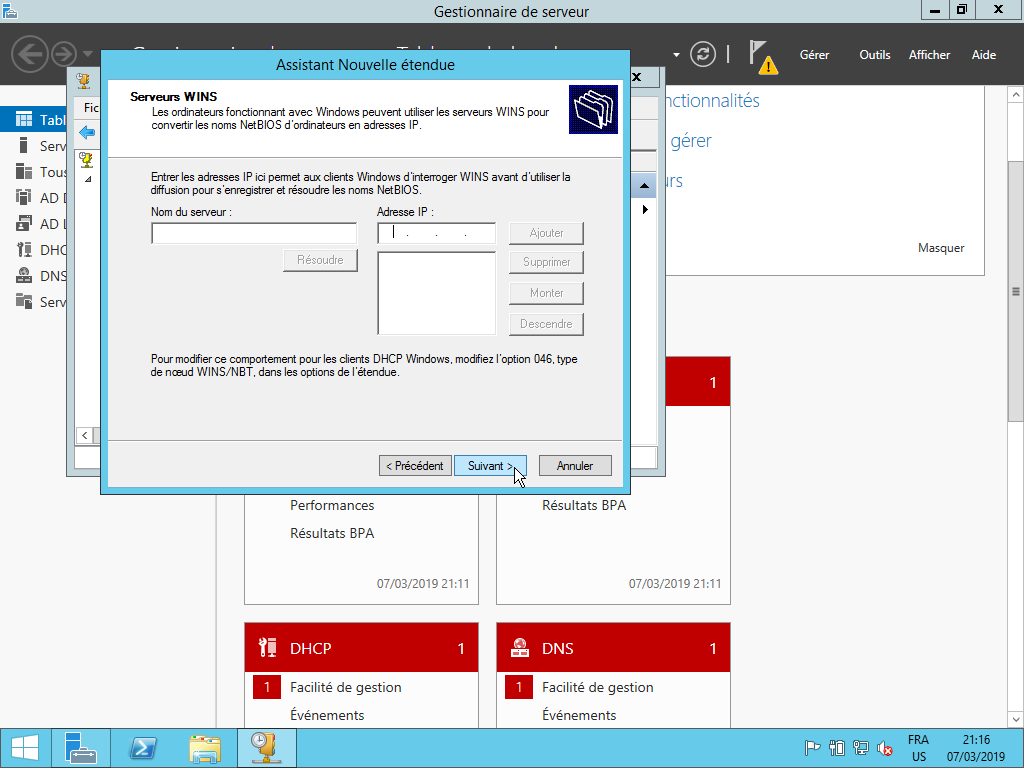
\includegraphics[scale=0.6]{WS2012_Screenshots/50.png}
        \caption{Serveurs WINS - Assistant Nouvelle étendue du Gestionnaire DHCP de Windows Server 2012}
        \label{WS2012_Screenshots/50}
    \end{center}
\end{figure}
\FloatBarrier

\newpage
Cocher l'option "\textit{Oui, je veux activer cette étendue maintenant}", puis cliquer sur \textit{Suivant} :
\begin{figure}[h!]
    \begin{center}
        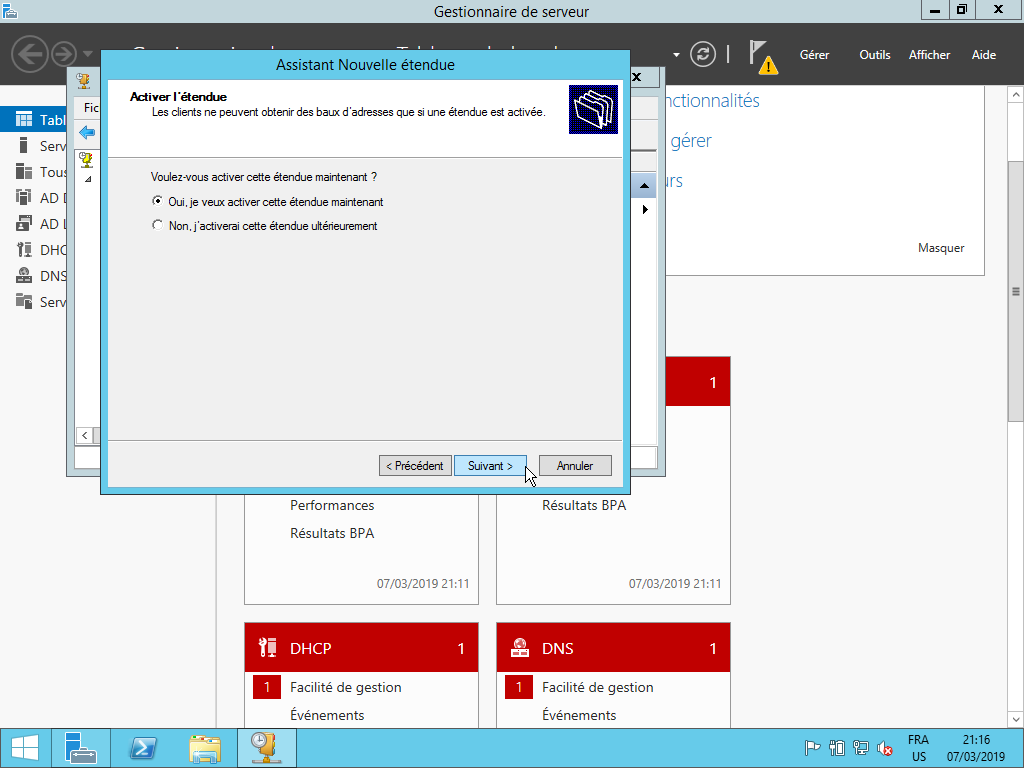
\includegraphics[scale=0.6]{WS2012_Screenshots/51.png}
        \caption{Activation de l'étendue - Assistant Nouvelle étendue du Gestionnaire DHCP de Windows Server 2012}
        \label{WS2012_Screenshots/51}
    \end{center}
\end{figure}
\FloatBarrier

\newpage
Cliquer sur \textit{Terminer} :
\begin{figure}[h!]
    \begin{center}
        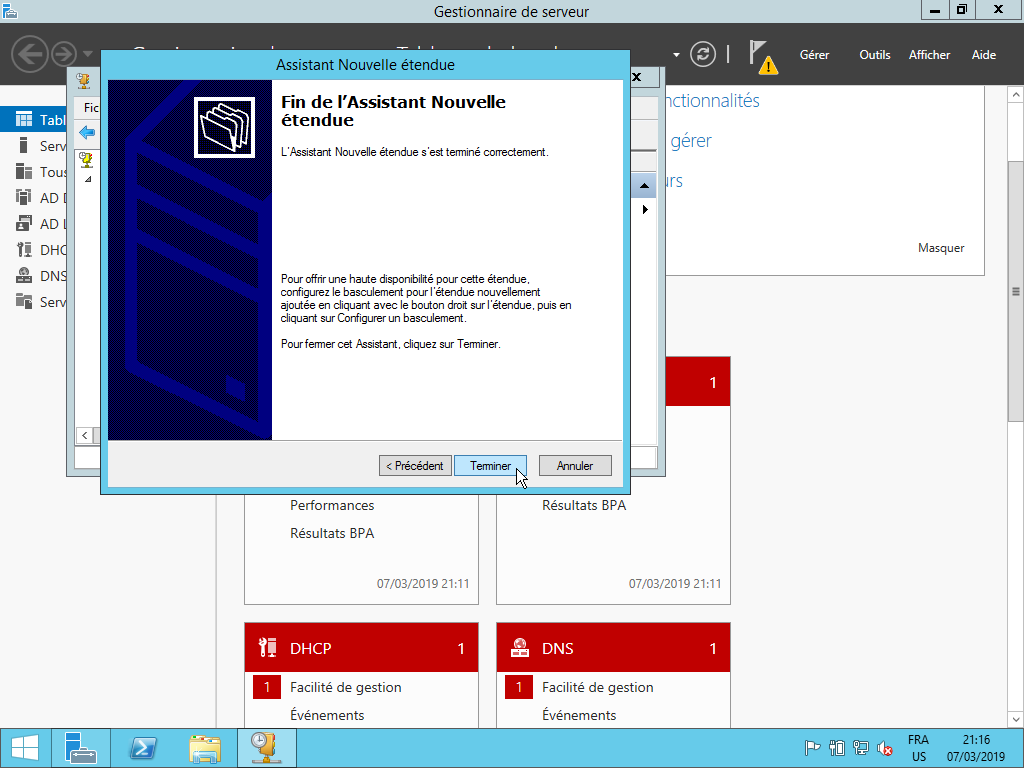
\includegraphics[scale=0.6]{WS2012_Screenshots/52.png}
        \caption{Fin de la nouvelle étendue - Assistant Nouvelle étendue du Gestionnaire DHCP de Windows Server 2012}
        \label{WS2012_Screenshots/52}
    \end{center}
\end{figure}
\FloatBarrier

\newpage
\subsection{Création de l'Active Directory}

Cliquer sur \textit{Outils}, puis cliquer sur \textit{Centre d'administration Active Directory} :
\begin{figure}[h!]
    \begin{center}
        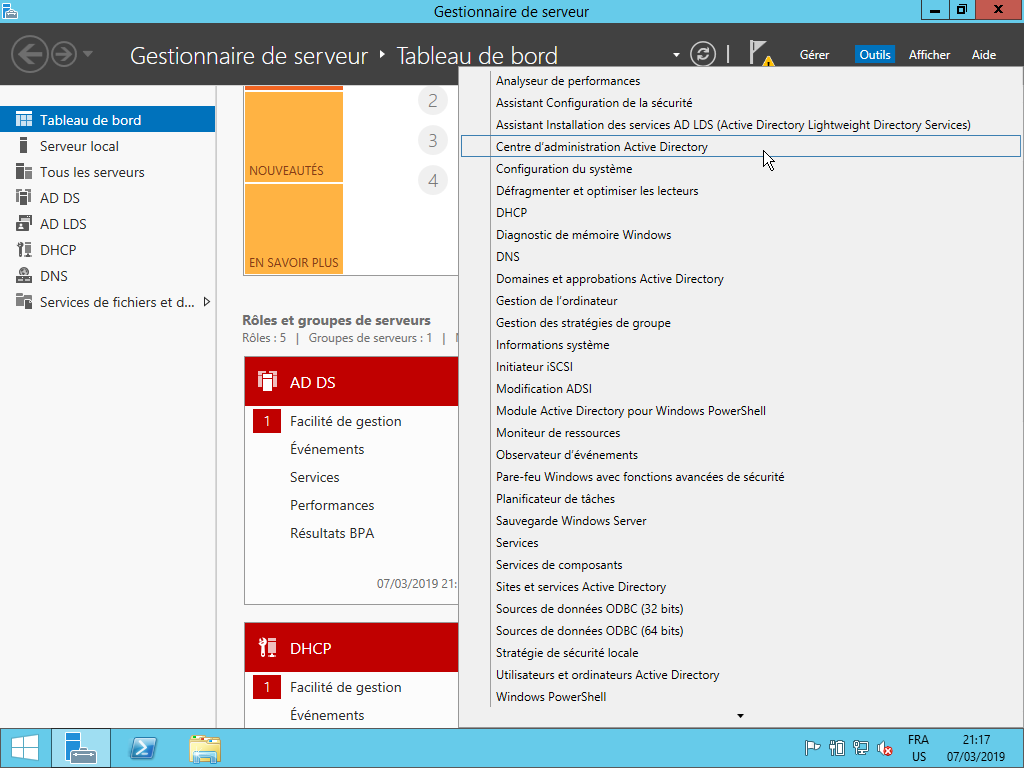
\includegraphics[scale=0.6]{WS2012_Screenshots/53.png}
        \caption{Centre d'administration Active Directory}
        \label{WS2012_Screenshots/53}
    \end{center}
\end{figure}
\FloatBarrier

\newpage
Dans l'encadré \textbf{Serveurs}, cliquer sur \textit{Autres...} :
\begin{figure}[h!]
    \begin{center}
        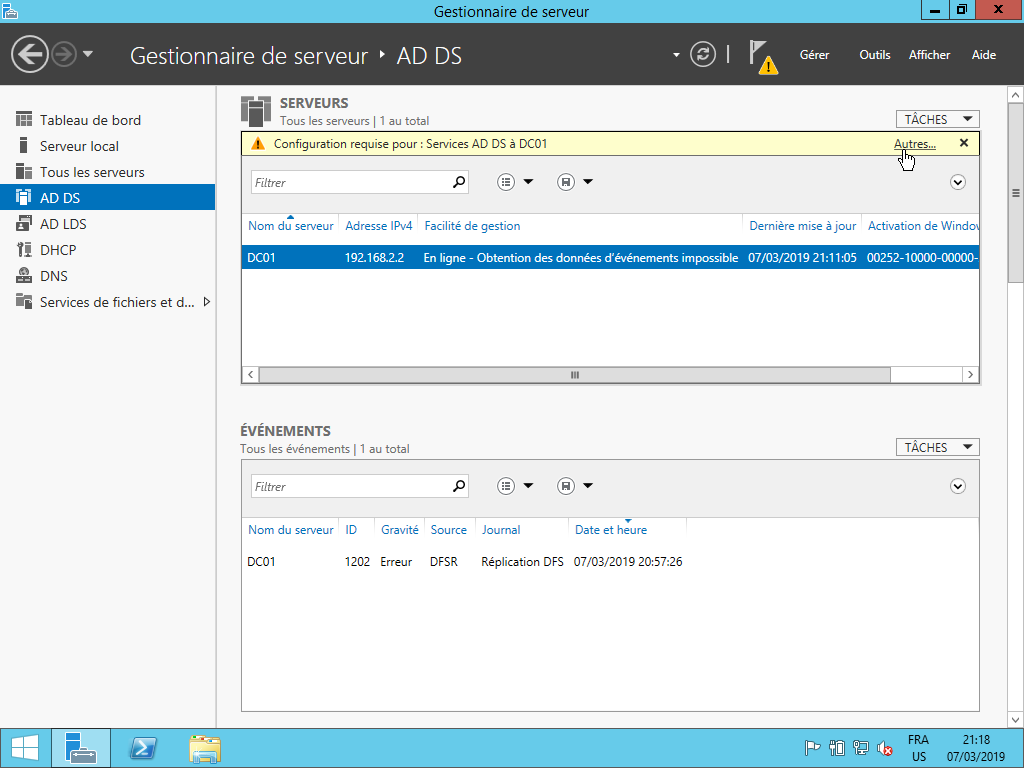
\includegraphics[scale=0.6]{WS2012_Screenshots/54.png}
        \caption{Configuration AD DS de Windows Server 2012}
        \label{WS2012_Screenshots/54}
    \end{center}
\end{figure}
\FloatBarrier

\newpage
Cliquer sur l'action \textit{Promouvoir ce serveur en contrôleur de domaine} :
\begin{figure}[h!]
    \begin{center}
        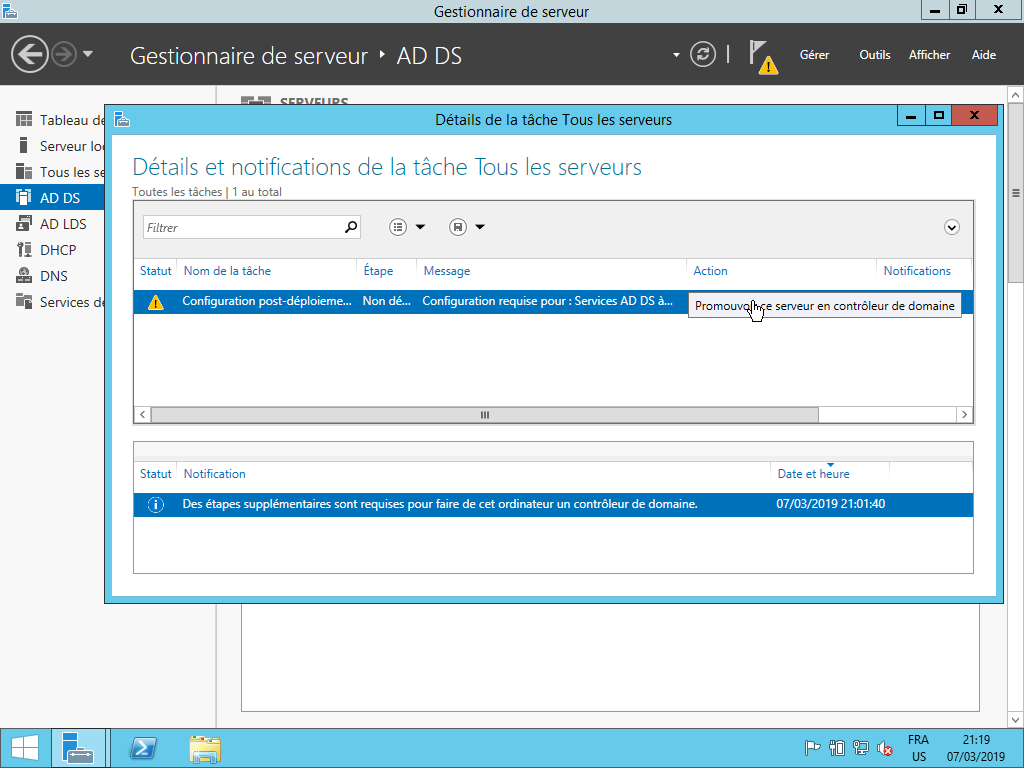
\includegraphics[scale=0.6]{WS2012_Screenshots/55.png}
        \caption{Configuration post-déploiement AD DS de Windows Server 2012}
        \label{WS2012_Screenshots/55}
    \end{center}
\end{figure}
\FloatBarrier

\newpage
Aller dans la section \textit{Configuration de déploiement} :
\begin{figure}[h!]
    \begin{center}
        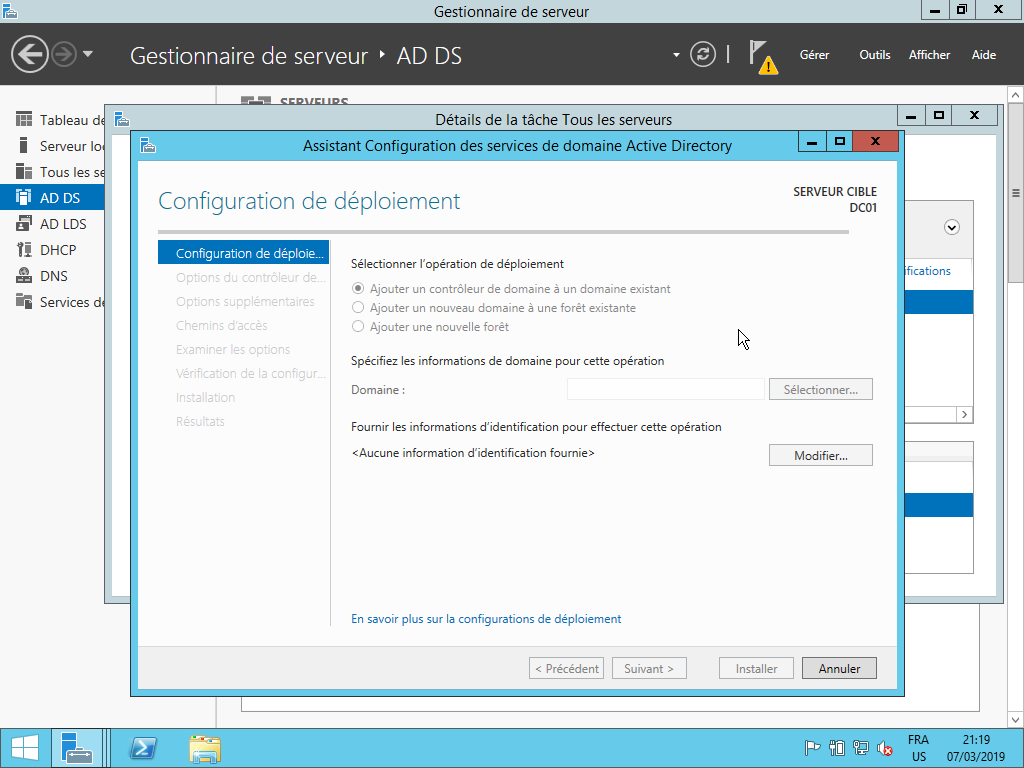
\includegraphics[scale=0.6]{WS2012_Screenshots/56.png}
        \caption{Configuration de déploiement - Configuration des services de domaine Active Directory de Windows Server 2012}
        \label{WS2012_Screenshots/56}
    \end{center}
\end{figure}
\FloatBarrier

\newpage
Cocher l'option "\textit{Ajouter une nouvelle forêt}", et entrer la valeur "\textit{EPITAF.local}" dans le champ \textit{Nom de domaine racine}. Cliquer sur \textit{Suivant} :
\begin{figure}[h!]
    \begin{center}
        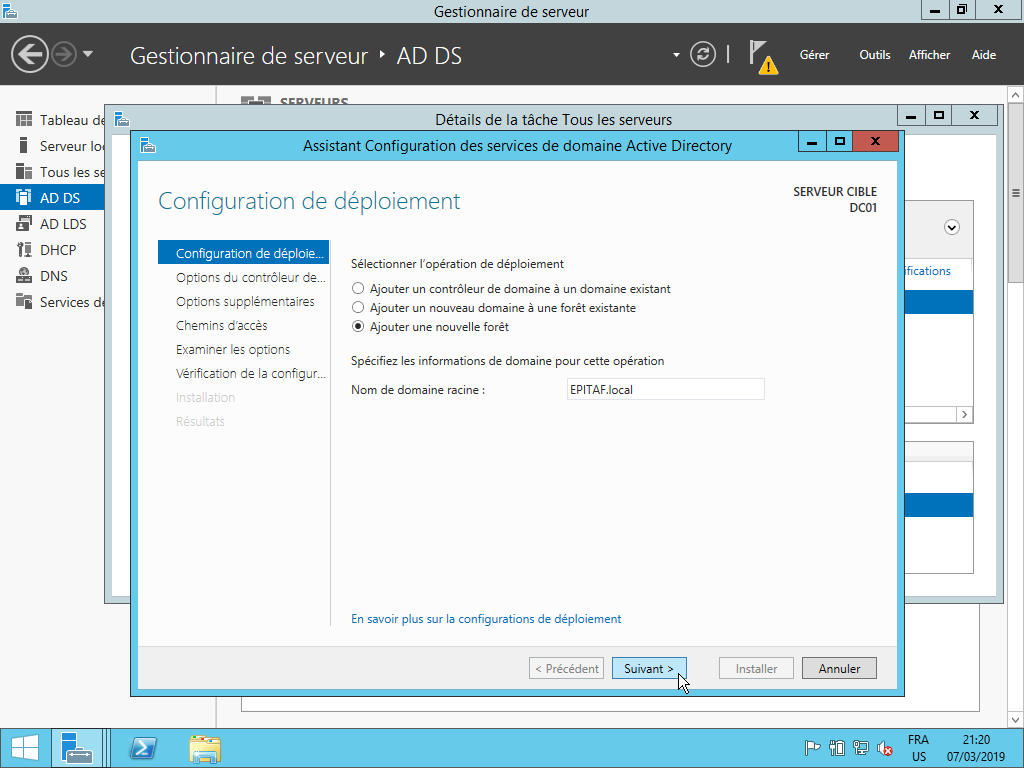
\includegraphics[scale=0.6]{WS2012_Screenshots/58.png}
        \caption{Ajout d'une nouvelle forêt - Configuration des services de domaine Active Directory de Windows Server 2012}
        \label{WS2012_Screenshots/58}
    \end{center}
\end{figure}
\FloatBarrier

\newpage
Aller dans la section \textit{Options du contrôleur de domaine}. Entrer un mot de passe respectant les bonne pratiques de sécurité, puis cliquer sur \textit{Suivant} :
\begin{figure}[h!]
    \begin{center}
        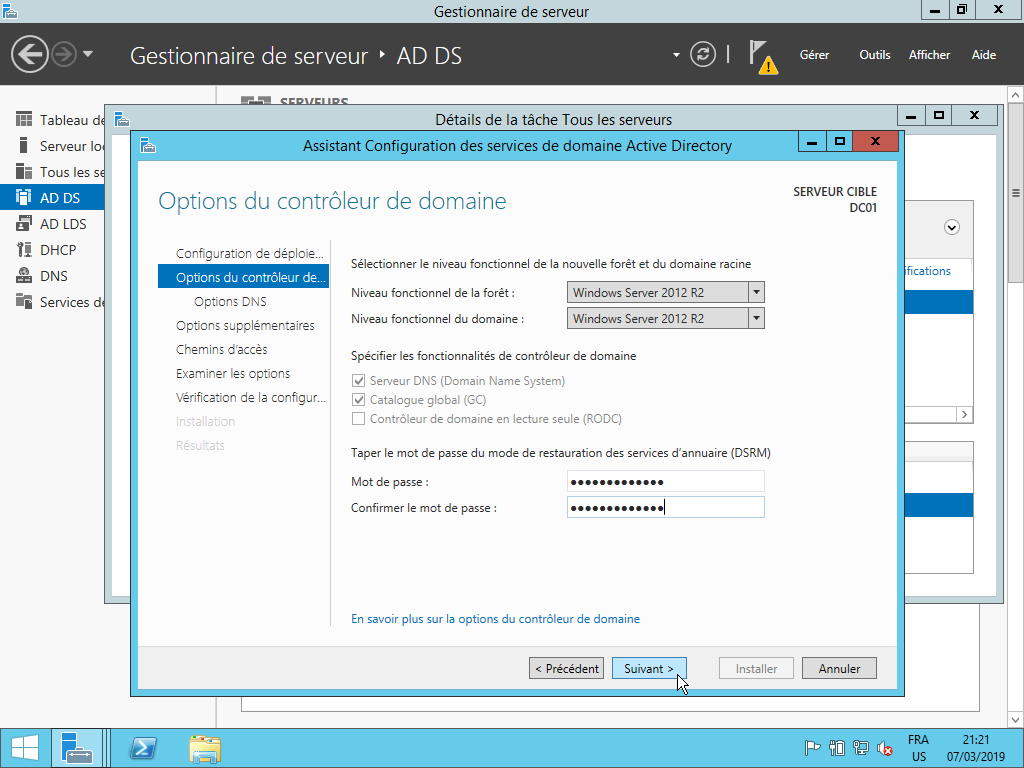
\includegraphics[scale=0.6]{WS2012_Screenshots/59.png}
        \caption{Options du contrôleur de domaine - Configuration des services de domaine Active Directory de Windows Server 2012}
        \label{WS2012_Screenshots/59}
    \end{center}
\end{figure}
\FloatBarrier

\newpage
Aller dans la section \textit{Options DNS}, puis cliquer sur \textit{Suivant} :
\begin{figure}[h!]
    \begin{center}
        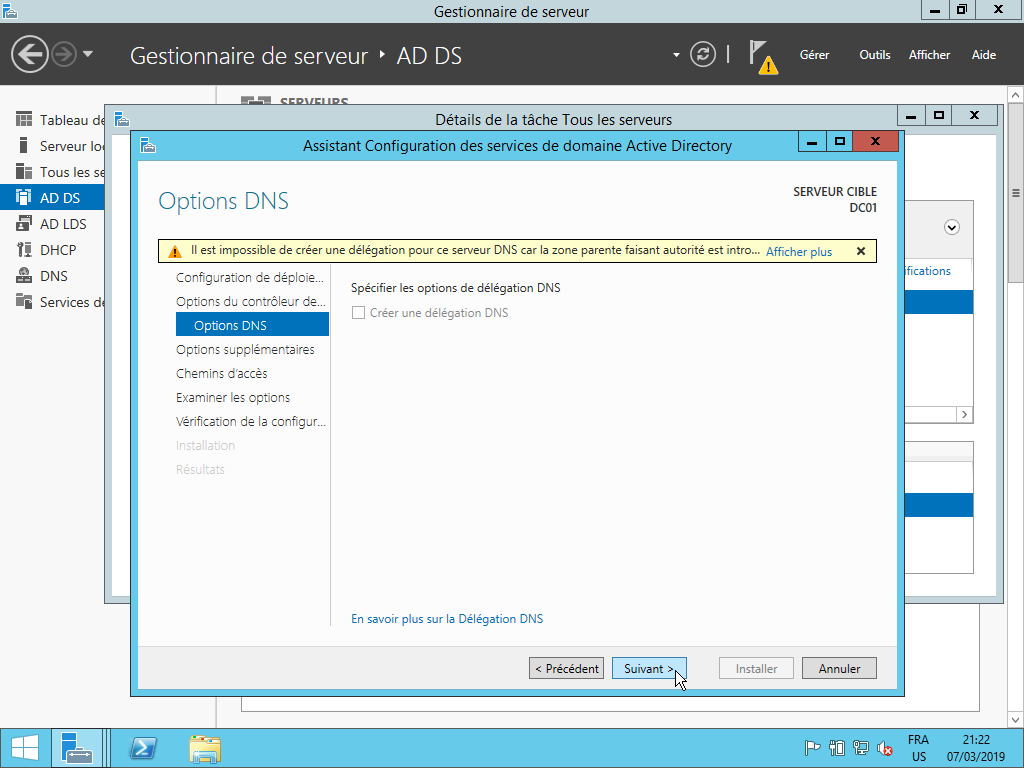
\includegraphics[scale=0.6]{WS2012_Screenshots/60.png}
        \caption{Options DNS - Configuration des services de domaine Active Directory de Windows Server 2012}
        \label{WS2012_Screenshots/60}
    \end{center}
\end{figure}
\FloatBarrier

\newpage
Aller dans la section \textit{Options supplémentaires}, puis cliquer sur \textit{Suivant} :
\begin{figure}[h!]
    \begin{center}
        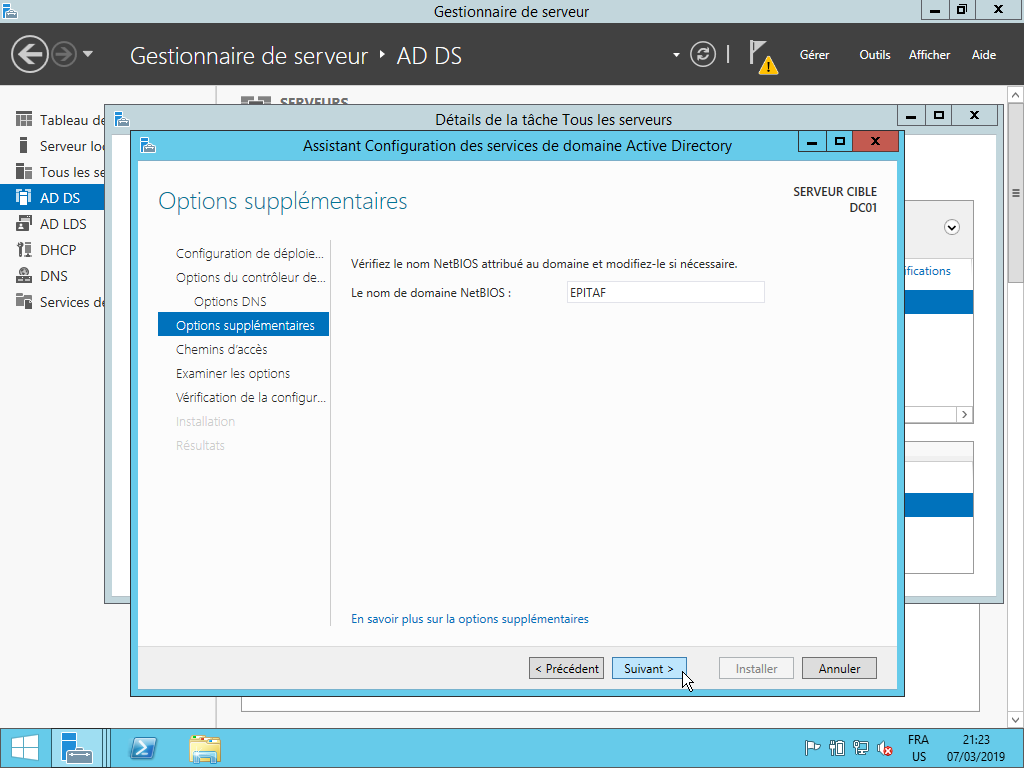
\includegraphics[scale=0.6]{WS2012_Screenshots/61.png}
        \caption{Options supplémentaires - Configuration des services de domaine Active Directory de Windows Server 2012}
        \label{WS2012_Screenshots/61}
    \end{center}
\end{figure}
\FloatBarrier

\newpage
Aller dans la section \textit{Chemins d'accès}, puis cliquer sur \textit{Suivant} :
\begin{figure}[h!]
    \begin{center}
        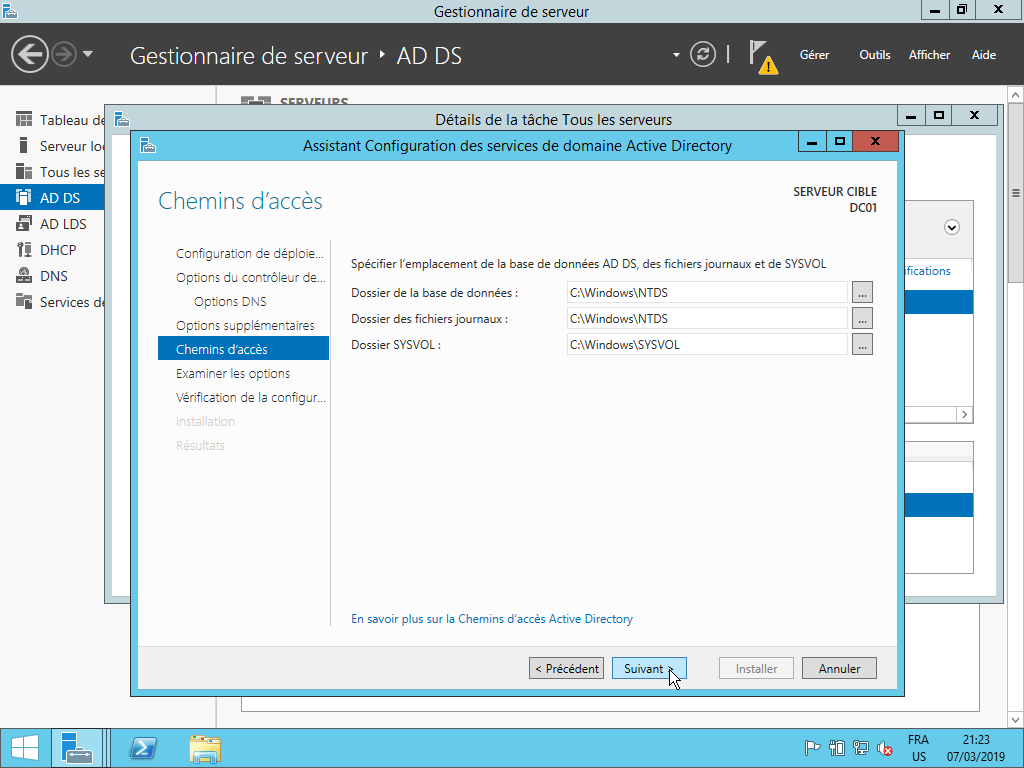
\includegraphics[scale=0.6]{WS2012_Screenshots/62.png}
        \caption{Chemins d'accès - Configuration des services de domaine Active Directory de Windows Server 2012}
        \label{WS2012_Screenshots/62}
    \end{center}
\end{figure}
\FloatBarrier

\newpage
Aller dans la section \textit{Examiner les options}, puis cliquer sur \textit{Suivant} :
\begin{figure}[h!]
    \begin{center}
        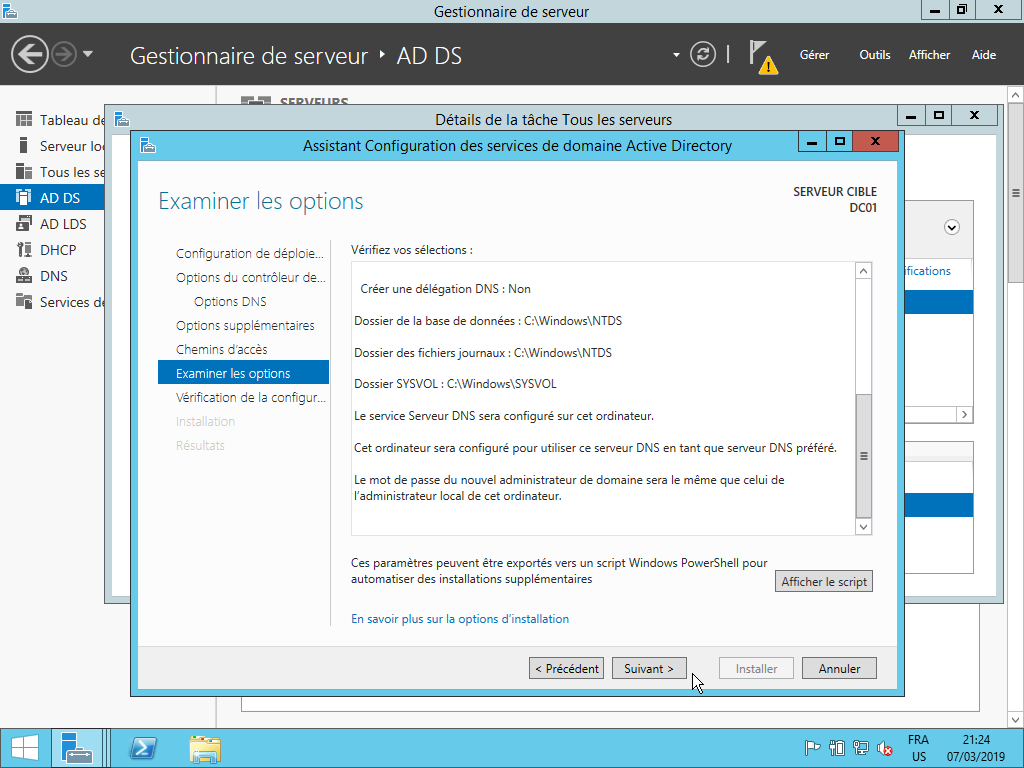
\includegraphics[scale=0.6]{WS2012_Screenshots/63.png}
        \caption{Examiner les options - Configuration des services de domaine Active Directory de Windows Server 2012}
        \label{WS2012_Screenshots/63}
    \end{center}
\end{figure}
\FloatBarrier

\newpage
Aller dans la section \textit{Vérification de la configuration requise}, puis cliquer sur \textit{Installer} :
\begin{figure}[h!]
    \begin{center}
        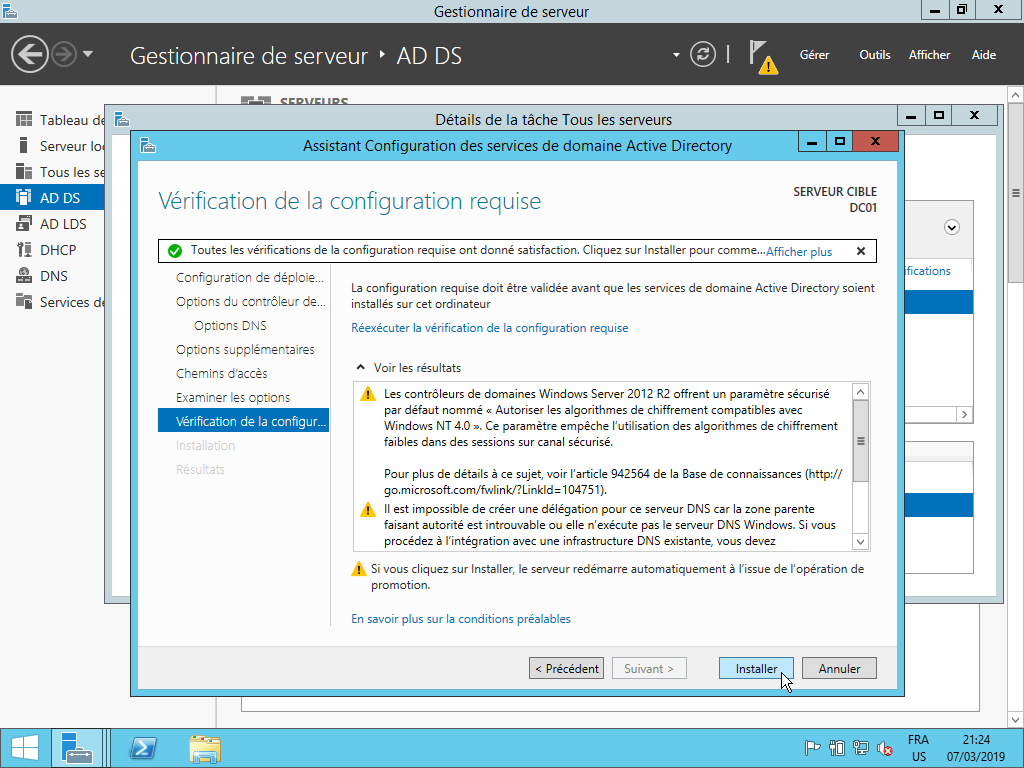
\includegraphics[scale=0.6]{WS2012_Screenshots/64.png}
        \caption{Vérification de la configuration requise - Configuration des services de domaine Active Directory de Windows Server 2012}
        \label{WS2012_Screenshots/64}
    \end{center}
\end{figure}
\FloatBarrier

\newpage
Une fois le serveur redémarré, se connecter au compte administrateur du domaine EPITAF.
\begin{figure}[h!]
    \begin{center}
        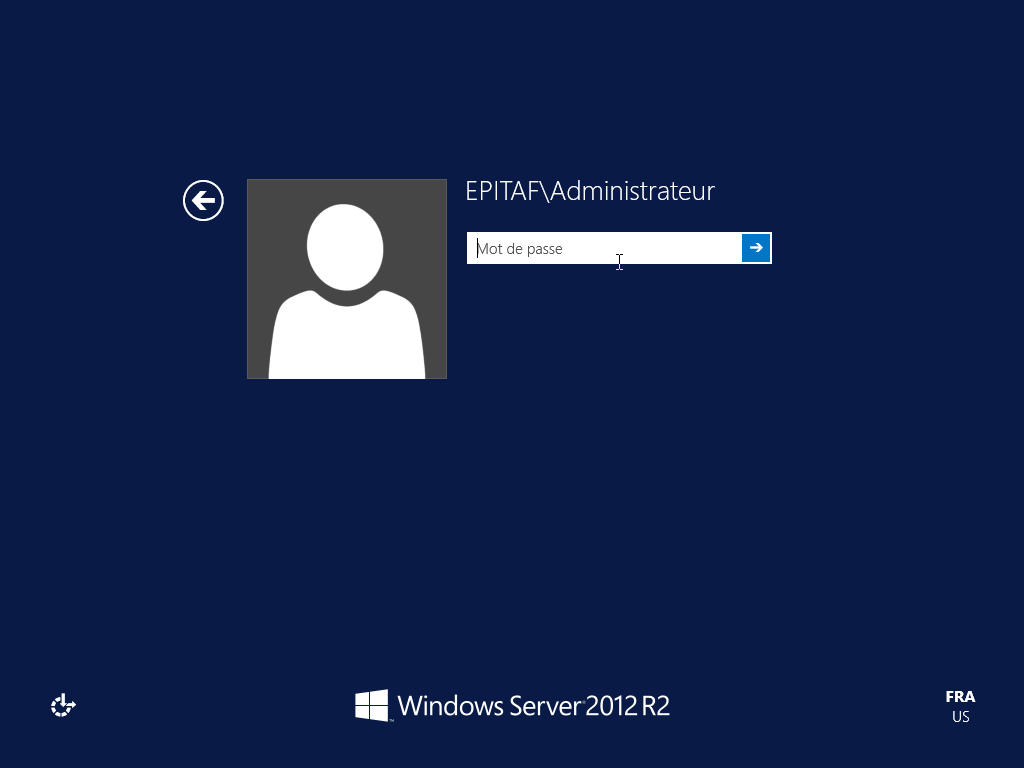
\includegraphics[scale=0.6]{WS2012_Screenshots/65.png}
        \caption{Accès au compte administrateur du domaine EPITAF de Windows Server 2012}
        \label{WS2012_Screenshots/65}
    \end{center}
\end{figure}
\FloatBarrier

\newpage
Dans le gestionnaire de serveur, aller dans la section \textbf{DHCP} via la colonne de gauche. Cliquer sur \textit{Autres...} dans l'encart jaune :
\begin{figure}[h!]
    \begin{center}
        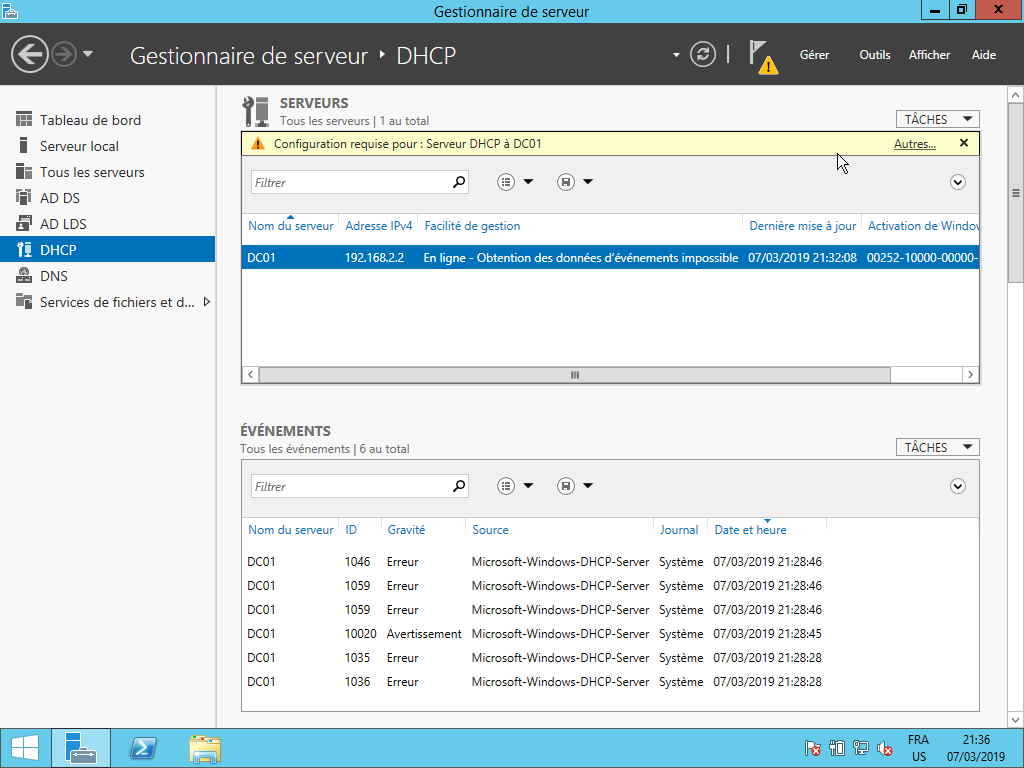
\includegraphics[scale=0.6]{WS2012_Screenshots/66.png}
        \caption{Configuration du serveur DHCP pour AD DS de Windows Server 2012}
        \label{WS2012_Screenshots/66}
    \end{center}
\end{figure}
\FloatBarrier

\newpage
Cliquer sur l'action "\textit{Terminer la configuration DHCP}" :
\begin{figure}[h!]
    \begin{center}
        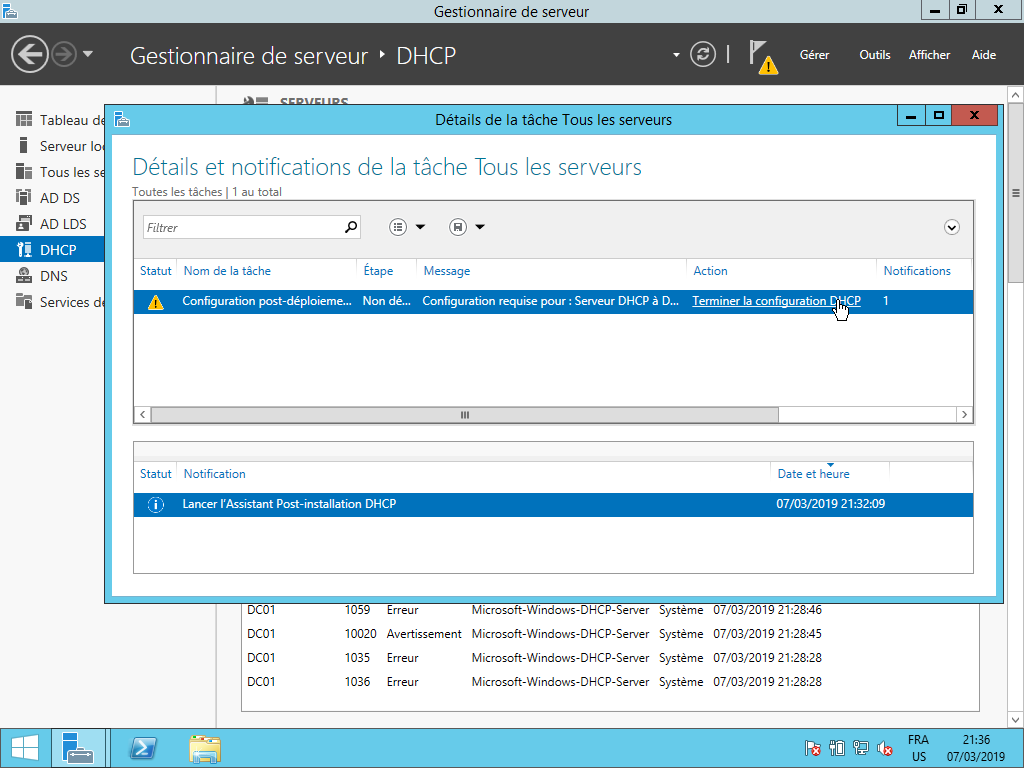
\includegraphics[scale=0.6]{WS2012_Screenshots/67.png}
        \caption{Configuration post-déploiement du serveur DHCP pour AD DS de Windows Server 2012}
        \label{WS2012_Screenshots/67}
    \end{center}
\end{figure}
\FloatBarrier

\newpage
Dans la section \textit{Description} cliquer sur \textit{Suivant} :
\begin{figure}[h!]
    \begin{center}
        \includegraphics[scale=0.6]{WS2012_Screenshots/68.png}
        \caption{Description - Assistant Configuration post-déploiement DHCP pour AD DS de Windows Server 2012}
        \label{WS2012_Screenshots/68}
    \end{center}
\end{figure}
\FloatBarrier

\newpage
Dans la section \textit{Autorisation}, cocher l'option "\textit{Utiliser les informations d'identification de l'utilisateur suivant}", pour l'utilisateur \texttt{EPITAF\textbackslash Administrateur}. Cliquer sur \textit{Valider} :
\begin{figure}[h!]
    \begin{center}
        \includegraphics[scale=0.6]{WS2012_Screenshots/69.png}
        \caption{Autorisation - Assistant Configuration post-déploiement DHCP pour AD DS de Windows Server 2012}
        \label{WS2012_Screenshots/69}
    \end{center}
\end{figure}
\FloatBarrier

\newpage
Dans la section \textit{Résumé} cliquer sur \textit{Fermer} :
\begin{figure}[h!]
    \begin{center}
        \includegraphics[scale=0.6]{WS2012_Screenshots/70.png}
        \caption{Résumé - Assistant Configuration post-déploiement DHCP pour AD DS de Windows Server 2012}
        \label{WS2012_Screenshots/70}
    \end{center}
\end{figure}
\FloatBarrier

\newpage
Cliquer sur \textit{Outils}, puis cliquer sur \textit{DHCP}. Ensuite, dérouler la section IPv4, et cliquer droit sur \textit{Options de serveur}, puis cliquer sur \textit{Configurer les options...} :
\begin{figure}[h!]
    \begin{center}
        \includegraphics[scale=0.6]{WS2012_Screenshots/71.png}
        \caption{Accès à la configuration des options de serveur DHCP de Windows Server 2012}
        \label{WS2012_Screenshots/71}
    \end{center}
\end{figure}
\FloatBarrier

\newpage
Cocher l'option \texttt{003 Routeur}. Dans le champ \textit{Adresse IP}, entrer l'adresse IP 192.168.2.1, puis cliquer sur \textit{Ajouter} :
\begin{figure}[h!]
    \begin{center}
        \includegraphics[scale=0.6]{WS2012_Screenshots/72.png}
        \caption{Paramétrage de l'option routeur du serveur DHCP de Windows Server 2012}
        \label{WS2012_Screenshots/72}
    \end{center}
\end{figure}
\FloatBarrier

\newpage
Cocher l'option \texttt{006 Servers DNS}. Dans le champ \textit{Adresse IP}, entrer l'adresse IP 192.168.2.2, puis cliquer sur \textit{Ajouter}. Enfin, cliquer sur \textit{OK} :
\begin{figure}[h!]
    \begin{center}
        \includegraphics[scale=0.6]{WS2012_Screenshots/73.png}
        \caption{Paramétrage de l'option DNS de Windows Server 2012}
        \label{WS2012_Screenshots/73}
    \end{center}
\end{figure}
\FloatBarrier

\newpage
\subsection{Ajout d'un utilisateur dans le domaine EPITAF}

Pour ajouter en toute sécurité un utilisateur dans notre domaine EPITAF, nous allons :
\begin{itemize}

\item Depuis le \textbf{Gestionnaire de serveur}, cliquer sur \textbf{Outils} puis sur \textbf{Utilisateurs et ordinateurs AD} ;
\begin{figure}[h!]
    \begin{center}
        \includegraphics[scale=0.20]{PC01/PC1.png}
        \caption{Accès aux utilisateurs et ordinateurs AD de Windows Server 2012}
    \end{center}
\end{figure}
\FloatBarrier

\item Dérouler le menu comme suit : \textbf{Utilisateurs et ordinateurs AD -> EPITAF.local -> Users}, cliquer droit sur \textbf{Users}. Dans le menu \textbf{Nouveau} cliquer sur \textbf{Utilisateur} ;
\begin{figure}[h!]
    \begin{center}
        \includegraphics[scale=0.21]{PC01/PC2.png}
        \caption{Ajout d'un utilisateur dans le domaine EPITAF de Windows Server 2012}
    \end{center}
\end{figure}
\FloatBarrier

\item Renseigner les champs puis cliquer sur \textbf{Suivant} ;
\begin{figure}[h!]
    \begin{center}
        \includegraphics[scale=0.23]{PC01/PC3.png}
        \caption{Initialisation d'un utilisateur dans le domaine EPITAF de Windows Server 2012}
    \end{center}
\end{figure}
\FloatBarrier

\item Renseigner le mot de passe de l'utilisateur puis cliquer sur \textbf{Suivant} ;
\begin{figure}[h!]
    \begin{center}
        \includegraphics[scale=0.23]{PC01/PC4.png}
        \caption{Initialisation du mot de passe d'un utilisateur dans le domaine EPITAF de Windows Server 2012}
    \end{center}
\end{figure}
\FloatBarrier

\item Vérifier les informations puis cliquer sur \textbf{Terminer}.
\begin{figure}[h!]
    \begin{center}
        \includegraphics[scale=0.20]{PC01/PC5.png}
        \caption{Fin de l'ajout d'un utilisateur dans le domaine EPITAF de Windows Server 2012}
    \end{center}
\end{figure}
\FloatBarrier
\end{itemize}

\newpage
\subsection{Ajout d'un ordinateur dans le domaine EPITAF}

Pour ajouter un ordinateur dans le domaine EPITAF, il faut :
\begin{itemize}
\item Dérouler le menu comme suit : \textbf{Utilisateurs et ordinateurs AD -> EPITAF.local -> Computers}, cliquer droit sur \textbf{Computers}. Dans le menu \textbf{Nouveau} cliquer sur \textbf{Ordinateur} ;
\begin{figure}[h!]
    \begin{center}
        \includegraphics[scale=0.21]{PC01/PC7.png}
        \caption{Ajout d'un ordinateur dans le domaine EPITAF de Windows Server 2012}
    \end{center}
\end{figure}
\FloatBarrier

\item Remplir les champs adéquats puis cliquer sur \textbf{Modifier...} ;
\begin{figure}[h!]
    \begin{center}
        \includegraphics[scale=0.21]{PC01/PC8.png}
        \caption{Initialisation du nouvel ordinateur sur Windows Server 2012}
    \end{center}
\end{figure}
\FloatBarrier

\item Renseigner le nom de l'utilisateur précédemment créé puis cliquer sur \textbf{OK} ;
\begin{figure}[h!]
    \begin{center}
        \includegraphics[scale=0.20]{PC01/PC9.png}
        \caption{Paramétrage de l'option DNS de Windows Server 2012}
    \end{center}
\end{figure}
\FloatBarrier

\item Cliquer sur \textbf{OK} :
\begin{figure}[h!]
    \begin{center}
        \includegraphics[scale=0.20]{PC01/PC10.png}
        \caption{Paramétrage de l'option DNS de Windows Server 2012}
    \end{center}
\end{figure}
\FloatBarrier
\end{itemize}